\documentclass[12pt,a4paper]{report}

% ── Encodage & langue ──────────────────────────────────────────────────────────
\usepackage[utf8]{inputenc}
\usepackage[T1]{fontenc}
\usepackage[french]{babel}

% ── Mise en page ───────────────────────────────────────────────────────────────
\usepackage[top=2.5cm, bottom=2.5cm, left=2.5cm, right=2.5cm]{geometry}
\usepackage{parskip}
\usepackage{setspace}
\usepackage{titlesec}

% Formatage des chapitres — réduction des espaces verticaux
\titleformat{\chapter}[display]
  {\normalfont\huge\bfseries}          % Format du titre
  {\chaptertitlename\ \thechapter}     % Étiquette (ex: "Chapitre 1")
  {5pt}                                % Espace entre l'étiquette et le titre
  {\Huge}                              % Format du titre lui-même
  []
  
% Réglage de l'espacement autour des titres de chapitres
\titlespacing*{\chapter}
  {0pt}       % Marge gauche (0 = pas de retrait)
  {-30pt}     % Espace vertical AVANT le titre (valeur négative = remonte)
  {10pt}      % Espace vertical APRÈS le titre (réduit)
\onehalfspacing

% ── Typographie ────────────────────────────────────────────────────────────────
\usepackage{lmodern}
\usepackage{microtype}

% ── Mathématiques ──────────────────────────────────────────────────────────────
\usepackage{amsmath, amssymb}

% ── Tableaux ───────────────────────────────────────────────────────────────────
\usepackage{booktabs}
\usepackage{tabularx}
\usepackage{array}
\usepackage{multirow}
\newcolumntype{L}[1]{>{\raggedright\arraybackslash}p{#1}}
\newcolumntype{C}[1]{>{\centering\arraybackslash}p{#1}}
\setlength{\tabcolsep}{10pt}
\renewcommand{\arraystretch}{1}
\usepackage{tablefootnote}

% ── Graphics ───────────────────────────────────────────────────────────────────
\usepackage{graphicx}
\usepackage{float}
\usepackage{wrapfig}
\usepackage{pdflscape}
\graphicspath{{img/}{../img/}{../../img/}{../../../img/}{../../../../img/}}


% ── Schémas ───────────────────────────────────────────────────────────────────
\usepackage{tikz}
\usetikzlibrary{arrows.meta, positioning, shapes.geometric, fit, calc}

% ── Code source ────────────────────────────────────────────────────────────────
\usepackage{listings}
\usepackage{xcolor}

\definecolor{codebg}{RGB}{245,245,245}
\definecolor{codeframe}{RGB}{200,200,200}
\definecolor{codecomment}{RGB}{100,100,100}
\definecolor{codestring}{RGB}{163,21,21}
\definecolor{codekeyword}{RGB}{0,0,255}
\definecolor{bertblue}{RGB}{37,99,235}
\definecolor{bertlightblue}{RGB}{219,234,254}

\lstset{
  backgroundcolor=\color{codebg},
  frame=single,
  rulecolor=\color{codeframe},
  basicstyle=\ttfamily\small,
  keywordstyle=\color{codekeyword}\bfseries,
  stringstyle=\color{codestring},
  commentstyle=\color{codecomment}\itshape,
  breaklines=true,
  showstringspaces=false,
  language=Python,
  literate=
    {é}{{\'{e}}}1 {è}{{\`{e}}}1 {ê}{{\^{e}}}1 {ë}{{\"e}}1
    {à}{{\`{a}}}1 {â}{{\^{a}}}1 {î}{{\^{i}}}1 {ô}{{\^{o}}}1
    {û}{{\^{u}}}1 {ù}{{\`{u}}}1 {ç}{{\c{c}}}1 {œ}{{\oe}}1
}

% ── Boîtes colorées ───────────────────────────────────────────────────────────
\usepackage{mdframed}
\usepackage{tcolorbox}
\tcbuselibrary{skins,breakable}
\definecolor{warnorange}{RGB}{234,88,12}
\definecolor{warnlight}{RGB}{255,237,213}

\newmdenv[
  backgroundcolor=blue!5,
  linecolor=blue!50!black,
  linewidth=1pt,
  innerleftmargin=10pt,
  innerrightmargin=10pt,
  innertopmargin=6pt,
  innerbottommargin=6pt,
  skipabove=8pt,
  skipbelow=8pt
]{remarque}

\newmdenv[
  backgroundcolor=orange!10,
  linecolor=orange!70!black,
  linewidth=1pt,
  innerleftmargin=10pt,
  innerrightmargin=10pt,
  innertopmargin=6pt,
  innerbottommargin=6pt,
  skipabove=8pt,
  skipbelow=8pt
]{avertissement}

\newtcolorbox{note}[1][]{
  colback=bertlightblue,colframe=bertblue,fonttitle=\bfseries,
  title={#1},breakable,arc=3pt,boxrule=0.8pt
}

\newtcolorbox{warn}[1][Attention]{
  colback=warnlight,colframe=warnorange,fonttitle=\bfseries,
  title={#1},breakable,arc=3pt,boxrule=0.8pt
}
\newtcolorbox{tip}[1][Astuce]{
  colback=tiplight,colframe=tipgreen,fonttitle=\bfseries,
  title={#1},breakable,arc=3pt,boxrule=0.8pt
}
\newtcolorbox{crit}[1][Problème critique]{
  colback=warnlight,colframe=red!70!black,fonttitle=\bfseries,
  title={#1},breakable,arc=3pt,boxrule=0.8pt
}

% ── Hyperliens ─────────────────────────────────────────────────────────────────
\usepackage[colorlinks=true, linkcolor=blue!70!black, urlcolor=blue!70!black]{hyperref}
\usepackage{bookmark}

% ── En-têtes / pieds de page ───────────────────────────────────────────────────
\usepackage{fancyhdr}
\setlength{\headheight}{14.2pt}
\addtolength{\topmargin}{-2.2pt}
\pagestyle{fancy}
\fancyhf{}
\lhead{\small Rapport Final}
\rhead{\small \leftmark}
\cfoot{\thepage}
\renewcommand{\headrulewidth}{0.4pt}
\newenvironment{motsclefs}
	{\begin{center}{\bfseries Mots-clefs\vspace{-\topsep}}\end{center}\quotation}
	{\endquotation}

% ── Profondeur de la table des matières ───────────────────────────────────────
\setcounter{tocdepth}{2}

% ══════════════════════════════════════════════════════════════════════════════
\begin{document}

% ── Page de titre ──────────────────────────────────────────────────────────────
\begin{titlepage}
  \centering

  \vspace{2cm}

  {\fontsize{22}{26}\selectfont\bfseries
    RAPPORT FINAL\\[0.3cm]
    Analyse de conversations patient-thérapeute\\[0.2cm]
    sur la santé mentale\par}
  {\color{blue!70!black}\rule{0.6\textwidth}{2pt}\par}
  \vspace{1cm}

  {\Large\bfseries Cahier des charges, Méthodologie,\\[0.2cm]
   Résultats et Analyses\par}

  \vspace{1.5cm}

  {\large\bfseries Encadrante : Lynda Tamine-Lechani\par}

  \vspace{1cm}

  {\normalsize\itshape
    Équipe projet :\\[0.3em]
    Ulysse Chasseigne, Idir Yahiaoui, Bantsoukissa Laure,\\
    Cruz Fernandes Diogo, Emin Belkheir, Esso-Y-N Trésor PANA,\\
    Logan Larroux, Yvan Sellier, Victor Blanquart--Blanchet, Lucas Da Silva\par}

  \vspace{1.5cm}
  {\fontsize{14}{18}\selectfont 1\textsuperscript{er} juin 2026\par}

  \vspace{1cm}
  \begin{tabular}[t]{c}
    \centering
    
\includegraphics[height=1.5cm]{universite-de-toulouse-logo.png}
    \hspace{10px}
    {
\includegraphics[height=1.5cm]{IRIT_logo.png}}
    \hspace{10px}
    \raisebox{0.70cm}{\normalsize [Info5.BE-SHS]\par}
  \end{tabular}

  \vfill

  {\color{blue!70!black}\rule{\textwidth}{0.4pt}\par}
  \vspace{0.4cm}
  {\small Code : \href{https://github.com/cypnet/Analyse-de-conversations-sur-la-sant-mentale-}{GitHub du projet}\par}
  \vspace{0.5cm}
\end{titlepage}

% ── Résumé ─────────────────────────────────────────────────────────────────────
\chapter*{Résumé}
\addcontentsline{toc}{chapter}{Résumé}

Ce rapport présente l'ensemble des travaux réalisés dans le cadre du projet d'analyse de conversations patient-thérapeute sur la santé mentale. Le projet s'articule autour de deux axes principaux : l'analyse exploratoire et la modélisation thématique des conversations (Étape 1), puis le développement d'un système d'analyse de sentiments et de question-réponse (Étape 2).

L'Étape 1 a permis d'explorer en profondeur le corpus de conversations à travers des analyses statistiques, lexicales et quatre méthodes de \textit{topic modeling} (lexique manuel, TF-IDF + K-Means, Word Embeddings et LDA). Les résultats montrent que les thématiques principales tournent autour des relations interpersonnelles, de l'anxiété et de la dépression.

L'Étape 2 a vu le développement parallèle d'un classificateur de sentiments (méthodes supervisées et non supervisées, incluant des approches BERT avancées) et d'un système de question-réponse basé sur la similarité sémantique. Les modèles BERT avec fine-tuning atteignent une accuracy de 83,43\%, surpassant significativement les méthodes classiques. Le système question-réponse, utilisant les représentations BERT, obtient un score de similarité de 0,702.

\begin{motsclefs}
\begin{center}
  Analyse de sentiments - Topic Modeling - BERT - NLP - Santé mentale - Système question-réponse - Word Embeddings - LDA - TF-IDF
\end{center}
\end{motsclefs}

% ── Table des matières ─────────────────────────────────────────────────────────
\tableofcontents

% ══════════════════════════════════════════════════════════════════════════════
% PARTIE I : CAHIER DES CHARGES
% ══════════════════════════════════════════════════════════════════════════════
\part{Cahier des charges et organisation}

\chapter{Contexte et objectifs du projet}

\section{Présentation générale}

La santé mentale est un enjeu majeur de la santé publique. Ce projet vise, dans un premier temps, à exploiter le jeu de données pour comprendre les types de conversations et leur structure, puis à analyser les sentiments des échanges afin de détecter les émotions et états psychologiques des patients. Ensuite, il se concentre sur l'accès et le traitement des conversations, en résumant les échanges et en identifiant les schémas linguistiques récurrents. Enfin, il prévoit le développement d'un système question-réponse, capable d'automatiser les interactions et fournir des réponses.

\section{Ressources utilisées}

\begin{itemize}
\item \href{https://www.kaggle.com/datasets/thedevastator/nlp-mental-health-conversations}{Ensemble de données Kaggle — NLP Mental Health Conversations}
\item \href{https://www.kaggle.com/datasets/suchintikasarkar/sentiment-analysis-for-mental-health/data}{Ensemble de données Kaggle — Sentiment Analysis for Mental Health}
\item \href{https://github.com/cypnet/Analyse-de-conversations-sur-la-sant-mentale-}{Page GitHub de l'équipe}
\end{itemize}

\chapter{Organisation et gouvernance du projet}

\section{Organisation des groupes}

L'organisation a évolué en deux phases :
\begin{itemize}
    \item \textbf{Étape 1 :} Travail individuel — chaque membre traite ses données de son côté pour en extraire des informations comparables.
    \item \textbf{Étape 2 :} Division en deux groupes distincts :
    \begin{itemize}
        \item \textbf{Groupe 1 :} Analyse des sentiments des conversations
        \item \textbf{Groupe 2 :} Question-réponse sur la santé mentale
    \end{itemize}
\end{itemize}

\section{Définition des rôles}
La direction du projet dans sa globalité est assurée par \textbf{Logan LARROUX}, 
qui supervise les deux groupes et garantit la cohérence des livrables.
Après constatation de l'ampleur des tâches à réaliser lors de l'étape 1, une bien meilleur organisation a été mise en place pour l'étape 2, avec des chefs de groupe dédiés à chaque axe d'analyse.

\subsection{Organisation étape 1: Exploration du jeu de données}
Lors de l'étape 1 chaque membre de l'équipe s'est vue assigné les mêmes tâches, afin d'en comparer et de contraster les résultats.

\textbf{Liste des membres: }
\begin{itemize}
    \item Ulysse Chasseigne
    \item Idir Yahiaoui
    \item Bantsoukissa Laure
    \item Cruz Fernandes Diogo
    \item Emin Belkheir
    \item Esso-Y-N Trésor PANA
    \item Logan Larroux
    \item Yvan Sellier
    \item Victor Blanquart-Blanchet
    \item Lucas Da Silva
\end{itemize}

\subsection{Organisation étape 2: Développement du système d'analyse de sentiments et de question-réponse}
Comme dit précédemment, l'étape 2 a été divisée en deux groupes distincts, avec des rôles clairement définis pour chaque membre.
En plus de cette séparation dans ses deux groupes, nous avons de nouveau séparé les tâches en sous-tâches, afin de mieux répartir le travail et d'assurer une meilleure coordination entre les membres.

\subsubsection{Groupe 1: Analyse des sentiments des conversations}
\textbf{Chef de groupe: Cruz Fernandes Diogo}
\begin{center}
\begin{tabular}{@{}cc@{}}
\toprule
\textbf{Sous-groupe 1} & \textbf{Sous-groupe 2} \\
\textbf{Méthode supervisée} & \textbf{Méthode non-supervisée} \\
\midrule
Diogo & Victor\\
Ulysse & Emin\\
Logan &  \\
\bottomrule
\end{tabular}
\end{center}

\subsubsection{Groupe 2: Question-réponse sur la santé mentale}
\textbf{Chef de groupe: Yahiaoui Idir}
\begin{center}
\begin{tabular}{@{}C{4.5cm}|C{4.5cm}|C{4.5cm}@{}}
\toprule
\textbf{Sous-groupe 1} & \textbf{Sous-groupe 2} & \textbf{Sous-groupe 3} \\
\textbf{Association Q\&A } & \textbf{Stratégie 1} & \textbf{Stratégie 2} \\
\textbf{pour chaque mot} & \textbf{Similarité} & \textbf{Similarité}\\
                         & \textbf{Question-Question} & \textbf{Question-Réponse}\\
\midrule
Lucas & Yvan & Laure\\
 & Trésor &  Idir\\
\bottomrule
\end{tabular}
\end{center}

\bigskip

\begin{note}[Petite précision]
Les étapes de développement de chaque groupe seront détaillées plus loin dans la deuxième et troisième partie du rapport.
\end{note}

\pagebreak

\subsection{Étape 2: Développement du système d'analyse de sentiments et de question-réponse}


% ══════════════════════════════════════════════════════════════════════════════
% PARTIE II : ÉTAPE 1
% ══════════════════════════════════════════════════════════════════════════════
\part{Étape 1 — Exploration du jeu de données}

\chapter{Méthodologie générale}

\textit{Objectif : Comprendre la structure du corpus et identifier les thématiques majeures.}

Le fichier \texttt{train.csv} comporte une grande base de données sur deux colonnes : la première est le patient conversant avec le psychologue (Context) et la seconde est la réponse du psychologue au patient (Response).

Cette première partie comporte :
\begin{itemize}
    \item \textbf{Nettoyage des données (Pré-traitement)} : Suppression de la ponctuation, tokenisation, lemmatisation et retrait des mots vides (\textit{stop-words}).
    \item \textbf{Analyse Statistique} : Création d'un tableau récapitulatif via des scripts Python (Pandas).
    \item \textbf{Analyse Lexicale} : Génération d'un dictionnaire lexical (n-grams) avec calcul des fréquences.
    \item \textbf{Modélisation et Extraction de Sujets (\textit{Topic Modeling})} : Quatre méthodes comparées.
\end{itemize}

\begin{figure}[H]
\begin{center}
\begin{tikzpicture}[
  scale=0.75,
  transform shape,
  node distance=8mm,
  >=Latex,
  box/.style={rounded corners, draw=blue!70!black, thick, fill=blue!5, align=center, text width=2.2cm, minimum height=0.9cm, inner sep=3pt, font=\small},
  method/.style={box, font=\footnotesize, text width=2cm, minimum height=0.8cm, node distance=4mm},
  group/.style={draw=orange!75!black, rounded corners, dashed, inner sep=4pt, thick},
  biggergroup/.style={group, draw=red!70!black, inner sep=18pt},
  arrow/.style={-Latex, thick, draw=blue!70!black}
]
  % ETAPE 1 ================================
  % Flux principal horizontal en dessous
  \node[box] (data) {\textbf{train.csv}};
  \node[box, below=of data] (clean) {Nettoyage};
  \node[box, below=of clean] (stats) {Analyse\\statistique};
  \node[box, below=of stats] (lex) {Analyse\\lexicale};
  \node[box, below=of lex] (topic) {Topic\\Modeling};

  \node[box, below=3cm of topic, text width=3cm] (conversations) {Étape 2\\Analyse et accès aux conversations};

  % Méthode de Nettoyage
  \node[method, left=1cm of data] (n1) {suppression\\ponctuation};
  \node[method, below=0.2cm of n1, text width=2.5cm] (n2) {lemmatisation};
  \node[method, left=0.2cm of n2] (n3) {tokenisation};
  \node[method, left=0.2cm of n1] (n4) {filtrage\\stopwords};
  \node[group, fit=(n1) (n2) (n3) (n4), label=above:\small\textbf{Comparaison des méthodes}] (methods1) {};

  % Méthodes d'analyse statistiques
  \node[method, right=1cm of data, text width=2.5cm] (s1) {Nombre de mots moyens};
  \node[method, right=of s1, text width=2.5cm] (s2) {Distribution des conversations};
  \node[method, below=0.2cm of s1, text width=2.5cm] (s3) {Mots les plus fréquents};
  \node[method, below=0.2cm of s2] (s4) {Hapax legomena};
  \node[method, below=0.2cm of s3, text width=3cm, xshift=1.6cm] (s5) {Corrélation patient/thérapeute};
  \node[group, fit=(s1) (s2) (s3) (s4) (s5), label=above:\small\textbf{Comparaison des mesures}] (methods2) {};

  % Méthodes d'analyse lexicale
  \node[method, left=1.5cm of lex, text width=3cm] (l1) {N-grams optimal\\Unigram ($N=1$)\\Bigram ($N=2$)\\Trigram ($N=3$)};
  \node[group, fit=(l1), label=above:\small\textbf{Comparaison des N-grams}] (methods3) {};

  % Méthodes de Topic Modeling
  \node[method, right=1cm of lex, yshift=0.2cm] (tm1) {Méthode 1\\Lexique métier};
  \node[method, right=0.2cm of tm1] (tm2) {Méthode 2\\TF-IDF};
  \node[method, below=0.2cm of tm1] (tm3) {Méthode 3\\Word2Vec};
  \node[method, below=0.2cm of tm2] (tm4) {Méthode 4\\LDA};
  % décaler le groupe entier vers la gauche
  \node[group, fit=(tm1) (tm2) (tm3) (tm4), label=above:\small\textbf{Comparaison des méthodes}] (methods4) {};

  % Flux principal horizontal
  \draw[arrow] (data) -- (clean);
  \draw[arrow] (clean) -- (stats);
  \draw[arrow] (stats) -- (lex);
  \draw[arrow] (lex) -- (topic);

  \draw[arrow] (topic) -- (conversations);

  % Flèches horizontales entre branches d'analyse
  \draw[arrow] (clean.west) -- ++(-0.4,0) -- ++(0,-0.3) -| (methods1.south);
  \draw[arrow] (stats.east) -- ++(0.4,0) -| (methods2.south);
  \draw[arrow] (lex.west) -- (methods3.east);
  \draw[arrow] (topic.east) -- ++(0.4,0) -- ++(0, -0.3) -| (methods4.south);

\end{tikzpicture}%
\label{fig:flowchart-etape1}
\caption{Pipeline détaillé de l'étape 1: Exploration du jeu de données}
\end{center}
\end{figure}

\pagebreak

\chapter{Pré-traitement des données}

\section{Nettoyage — Structure générale}

Avant toute analyse, plusieurs étapes de nettoyage ont été appliquées dans l'ordre suivant.

\textbf{Suppression des cellules vides et des doublons.}
Les lignes contenant des valeurs nulles dans les colonnes \texttt{Context} ou \texttt{Response}
ont été supprimées, ainsi que les lignes entièrement dupliquées.

\textbf{Filtrage des textes non-anglais.}
Le corpus contenait des phrases en espagnol. La bibliothèque \texttt{langdetect} a été utilisée
pour détecter la langue de chaque ligne et ne conserver que les textes identifiés comme anglais.
Cette détection est effectuée au niveau de la phrase entière, ce qui est bien plus fiable qu'une
détection mot par mot.

\begin{lstlisting}
from langdetect import detect, LangDetectException

def is_english_text(text):
    try:
        return detect(str(text)) == 'en'
    except LangDetectException:
        return True  # texte trop court -> on garde

mask = df['Context'].apply(is_english_text) \
     & df['Response'].apply(is_english_text)
df = df[mask].reset_index(drop=True)
\end{lstlisting}

\textbf{Normalisation.}
Tous les textes ont été passés en minuscules afin d'éviter que \textit{"Toto"} et \textit{"toto"}
soient traités comme deux mots distincts. Les espaces insécables (\texttt{\textbackslash xa0}),
fréquents dans des données extraites du web, ont également été supprimés.

\subsection{Tokenisation}

La tokenisation consiste à découper chaque phrase en unités élémentaires appelées
\textit{tokens}. La bibliothèque \textbf{spaCy} (\texttt{en\_core\_web\_sm}) a été utilisée
pour cette étape, via \texttt{nlp.pipe()} afin de traiter les données en batch et réduire le
temps de traitement.

\subsection{Suppression de la ponctuation et des mots vides}
\label{stopwords}

Les \textit{stopwords} (mots vides) sont des mots sans réelle signification sémantique
(pronoms, adverbes, mots de liaison). spaCy les identifie automatiquement via l'attribut
\texttt{token.is\_stop}. Les tokens de ponctuation ont été supprimés de la même façon avec
\texttt{token.is\_punct}.

Des mots trop génériques mais non reconnus comme stopwords ont également été filtrés
manuellement, voici deux exemple de listes d'extra\_stopwords utilisées par Logan et Lucas:

\begin{lstlisting}
# Exemple - Logan
extra_stopwords = {
    "feel", "like", "want", "know", "time",
    "thing", "good", "need", "year", "think",
    "tell", "say", "come", "go"
}
\end{lstlisting}

\begin{lstlisting}
# Exemple - Lucas
mots_inutiles = set([
    "i", "me", "my", "myself", "we", "our", "ours", "ourselves",
    # ... [liste complete dans le notebook]
    "there", "back", "even", "every", "years", "told", "going", "still"
])
\end{lstlisting}

\subsection{Lemmatisation}

La lemmatisation transforme chaque mot en sa forme de base (\textit{"running"} $\rightarrow$
\textit{"run"}, \textit{"better"} $\rightarrow$ \textit{"good"}). Cette étape réduit
drastiquement le nombre de tokens distincts et regroupe les formes similaires. Elle permet également
de filtrer les URLs, emails et chiffres dans une seule passe:

\begin{lstlisting}
df["Context_clean"] = [
    [
        token.lemma_
        for token in doc
        if not token.is_stop
        #...et autres filtres (is_punct, is_url, is_email, etc.)
        and token.lemma_ not in extra_stopwords
    ]
    for doc in docs_context
]
\end{lstlisting}

\begin{note}[Remarque importante]
  \texttt{spaCy} lemmatise différemment selon le contexte grammatical. Par exemple,
  \textit{"feeling"} utilisé comme nom reste tel quel au lieu d'être ramené à \textit{"feel"}.
  C'est pourquoi \textit{"feel"} a été retiré manuellement des extra\_stopwords pour éviter
  les doublons sémantiques.
\end{note}



\section{Nettoyage — Approches comparées}

Puisque ce pipeline n'a pas était imposé, chaque membre a pu appliquer son propre pré-traitement, avec des niveaux de filtrage différents.
Prennons l'exemple de deux approches contrastées, celle d'Emin et celle de Diogo.

\subsection{Approche minimaliste (Emin)}

Celle-ci est la plus simple, elle se limite à la suppression des lignes vides et au reset de l'index.
Le résultat est un nombre de patients et de thérapeutes plus élevé, mais avec un risque de bruit plus important dans les données.

\begin{lstlisting}
# Suppression des lignes vides
df = df.dropna(how='all')
df = df.dropna(subset=['Context'])
df = df.dropna(subset=['Response'])
df = df.reset_index(drop=True)
\end{lstlisting}

\subsection{Approche étendue (Diogo)}
Un version beaucoup plus étendu est celle de Diogo, qui inclut un nettoyage plus poussé du texte, 
ainsi qu'un filtrage pour ne garder que les conversations en anglais.\\
Cette approche réduit le nombre de patients et de thérapeutes uniques, 
mais améliore la qualité des données en éliminant les réponses non pertinentes ou 
dans une langue différente.

Son pipeline est donc le suivant:
\begin{itemize}
 \item Nettoyage du texte : suppression de la ponctuation, des caractères spéciaux, des espaces multiples, et conversion en minuscules.
 \item Filtrage linguistique : utilisation de la bibliothèque \texttt{langdetect} pour ne conserver que les conversations en anglais.
 \item Suppression des stop-words : retrait des mots vides courants en anglais pour se concentrer sur les termes significatifs.
 \item Suppression des doublons : élimination des conversations identiques pour éviter les biais dans les analyses statistiques.
 \item Réinitialisation de l'index : après les filtrages, l'index est réinitialisé pour une meilleure gestion des données.
\end{itemize}

% \begin{lstlisting}
% stop_words = set(stopwords.words('english'))

% def clean_text(text):
%     text = str(text).lower()
%     text = re.sub(r"[\r\n]+", " ", text)
%     text = re.sub(r"[^a-z0-9\s]", "", text)
%     text = re.sub(r"\s+", " ", text)
%     words = text.strip().split()
%     words = [w for w in words if w not in stop_words]
%     return " ".join(words)

% def is_english(text):
%     try:
%         return detect(str(text)) == 'en'
%     except:
%         return False

% df = df.dropna(subset=["Response"])
% df = df.drop_duplicates(subset=["Context", "Response"], keep="first")
% df['Context'] = df['Context'].apply(clean_text)
% df['Response'] = df['Response'].apply(clean_text)
% mask = df['Context'].apply(is_english) & df['Response'].apply(is_english)
% df = df[mask].reset_index(drop=True)
% \end{lstlisting}

\begin{warn}[Lemmatisation et tokenisation]
L'application de la lemmatisation (et de la tokenisation) pour l'analyse du texte a été un débat au seins de l'équipe.
La grande majorité de l'équipe a décider de ne pas l'appliquer lors de l'analyse statistique et lexicale du corpus, 
afin de conserver les formes originales des mots.
\end{warn}

\section{Résultats}

\subsection{Nombre de patients uniques}

\begin{center}
\begin{tabular}{@{}L{1.5cm}lL{5cm}L{4cm}@{}}
\toprule
\textbf{Résultat} & \textbf{Nb. Membres} & \textbf{Nom Membres} & \textbf{Méthode} \\
\midrule
995 & 8 personnes & Ulysse - Emin - Victor - Laure - Trésor - Yvan - Idir - Lucas & Sans prétraitement \\
819 & 1 personne  & Logan & Prétraitement + filtre espagnol \\
796 & 1 personne  & Diogo & Prétraitement + filtre espagnol \\
\bottomrule
\end{tabular}
\end{center}

\subsection{Nombre de thérapeutes uniques}

\begin{center}
\begin{tabular}{@{}llL{5cm}l@{}}
\toprule
\textbf{Résultat} & \textbf{Nb. Membres} & \textbf{Nom Membres} & \textbf{Méthode} \\
\midrule
2 479 & 6 personnes & Emin - Victor - Idir - Laure - Yvan - Lucas & Sans prétraitement \\
2 472 & 1 personne  & Ulysse & Léger prétraitement \\
2 409 & 1 personne  & Logan & Prétraitement complet \\
$\geq 12$ & 1 personne & Diogo & Pattern matching \\
\bottomrule
\end{tabular}
\end{center}

\begin{warn}[Limite importante]
Les valeurs autour de 2 400--2 479 correspondent très probablement au nombre de lignes/réponses dans le fichier, et non au nombre réel de thérapeutes distincts. En l'absence d'identifiant unique (ID), il est impossible de différencier les thérapeutes entre eux avec certitude.
\end{warn}

\subsection{Nombre de mots moyen par patient / thérapeute}

\begin{center}
\begin{tabular}{ll|ll}
\toprule
\multicolumn{2}{c|}{\textbf{Côté patients}} & \multicolumn{2}{c}{\textbf{Côté thérapeutes}} \\
\textbf{Membre} & \textbf{Mots moyens} & \textbf{Membre} & \textbf{Mots moyens} \\
\midrule
Victor & 66,86 & Emin   & 177,2 \\
Emin   & 55,2  & Victor & 140,2 \\
Idir   & 24,8  & Idir   &  84,8 \\
Lucas  & 21,3  & Lucas  &  82,4 \\
Logan  & 16,3  & Logan  &  60,1 \\
\bottomrule
\end{tabular}
\end{center}

\begin{note}[Interprétation]
  On observe un rapport allant du simple au quadruple selon le niveau de filtrage.
  Dans chaque cas, \textbf{les thérapeutes ont tendance à produire des réponses plus longues que les patients}, ce qui est cohérent avec la nature de leur rôle dans la conversation.
\end{note}

\begin{figure}[H]
  \begin{center}
  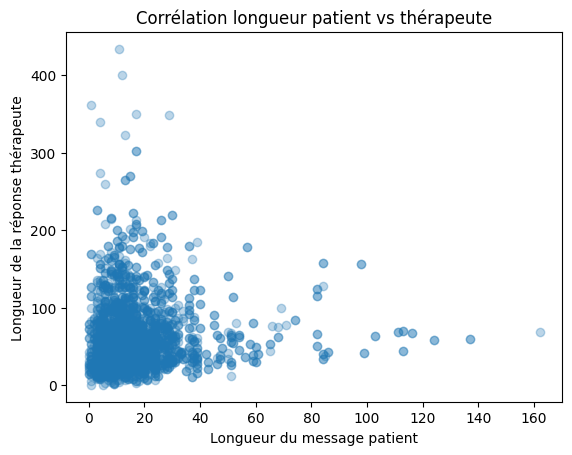
\includegraphics[width=0.50\textwidth]{correlationPatientVSTherapeute_Logan.png}
  \caption{Corrélation entre le nombre de mots côté patient et côté thérapeute — Logan}
  \end{center}
\end{figure}

\bigbreak

Maintenant que nous avons une idée de la structure générale du corpus, nous allons pouvoir nous pencher plus en détail sur les \textbf{thématiques abordées dans les conversations}, 
à travers une analyse lexicale afin de mieux comprendre les sujets centraux des échanges.

\chapter{Analyse lexicale et statistique}

\section{Mots les plus fréquents}
La fréquence des mots les plus utilisés dans les conversations peut révéler les thématiques centrales abordées par les patients et les thérapeutes.
Cependant, \textbf{il est crucial de filtrer les mots vides} (stop-words) pour éviter que des termes génériques ne dominent l'analyse.
\subsection{Sans filtrage renforcé}
Ulysse, Emin, Victor, Idir, Trésor et Yvan ont appliqué un filtrage minimal, ce qui a permis de conserver des mots très fréquents mais peu informatifs.
\begin{center}
\begin{tabular}{lll}
\toprule
\textbf{Côté patients} & \textbf{Côté thérapeutes} & \textbf{Global} \\
\midrule
\textit{im, feel, dont} & \textit{feel, may, help, like} & \textit{feel, like, may} \\
\bottomrule
\end{tabular}
\end{center}

\subsection{Avec filtrage renforcé}
Diogo, Logan, Laure et Lucas eux ont appliqué un filtrage plus poussé, en retirant des mots génériques comme \textit{feel}, \textit{like}, \textit{may}, qui sont très fréquents mais peu spécifiques.
\begin{center}
\begin{tabular}{lll}
\toprule
\textbf{Côté patients} & \textbf{Côté thérapeutes} & \textbf{Global} \\
\midrule
\textit{relationship, love, anxiety} & \textit{relationship, like} & \textit{relationship, help} \\
\bottomrule
\end{tabular}
\end{center}

\subsection{Interprétation}

\begin{itemize}
  \item \textbf{Sans filtrage renforcé} $\rightarrow$ expressions émotionnelles brutes des patients (\textit{feel}, \textit{love}) et posture d'aide des thérapeutes (\textit{may}, \textit{help}, \textit{would}).
  \item \textbf{Avec filtrage renforcé} $\rightarrow$ thématiques explicites : \textit{relationship}, \textit{anxiety}, \textit{love} côté patient ; \textit{relationship} côté thérapeute.
\end{itemize}

\begin{note}[Remarque]
Ces résultats confirment que le corpus est centré sur les relations interpersonnelles, sujet le plus fréquent, couplé à des états psychologiques comme l'anxiété.
\end{note}

\section{Analyse lexicale — N-grams}

\subsection{Définition}

Un \textbf{n-gram} est une séquence de $n$ mots consécutifs dans un texte. Cette approche
permet de capturer non seulement les mots isolés, mais aussi les associations de mots fréquentes.
\begin{itemize}
  \item \textbf{Unigram (n=1)} : mots individuels, ex. \textit{"anxiety"}, \textit{"depression"}.
  \item \textbf{Bigram (n=2)} : paires de mots, ex. \textit{"mental health"}, \textit{"feel like"}.
  \item \textbf{Trigram (n=3)} : triplets de mots, ex. \textit{"feel like cry"}, \textit{"family support system"}.
  \item ainsi de suite\dots
\end{itemize}
\vspace{1px}

Dans notre travail, nous allons devoir repérer des formulations récurrentes qui ont du sens:

\begin{table}[h]
\centering
\begin{tabularx}{\textwidth}{lXX}
\toprule
\textbf{Type} & \textbf{Exemple} & \textbf{Interprétation} \\
\midrule
Unigram (n=1) & \textit{anxiety} (fréq. 342) & Thème dominant \\
Bigram  (n=2) & \textit{mental health} (fréq. 87) & Expression caractéristique \\
Trigram (n=3) & \textit{feel like cry} (fréq. 54) & Patron de détresse \\
\bottomrule
\end{tabularx}
\caption{Exemples de n-grams et leur interprétation}
\end{table}

\subsection{Choix du n optimal}

Il n'existe pas de valeur universelle pour $n$. Deux indicateurs ont été utilisés pour guider
ce choix :

\begin{itemize}
  \item \textbf{Fréquence moyenne} : si elle chute sous un seuil de 5, les n-grams sont trop
        rares pour être statistiquement significatifs.
  \item \textbf{Pourcentage d'hapax} : si plus de 70\,\% des n-grams n'apparaissent qu'une
        seule fois, la taille $n$ est trop grande pour le corpus.
\end{itemize}

\begin{figure}[h]
\centering
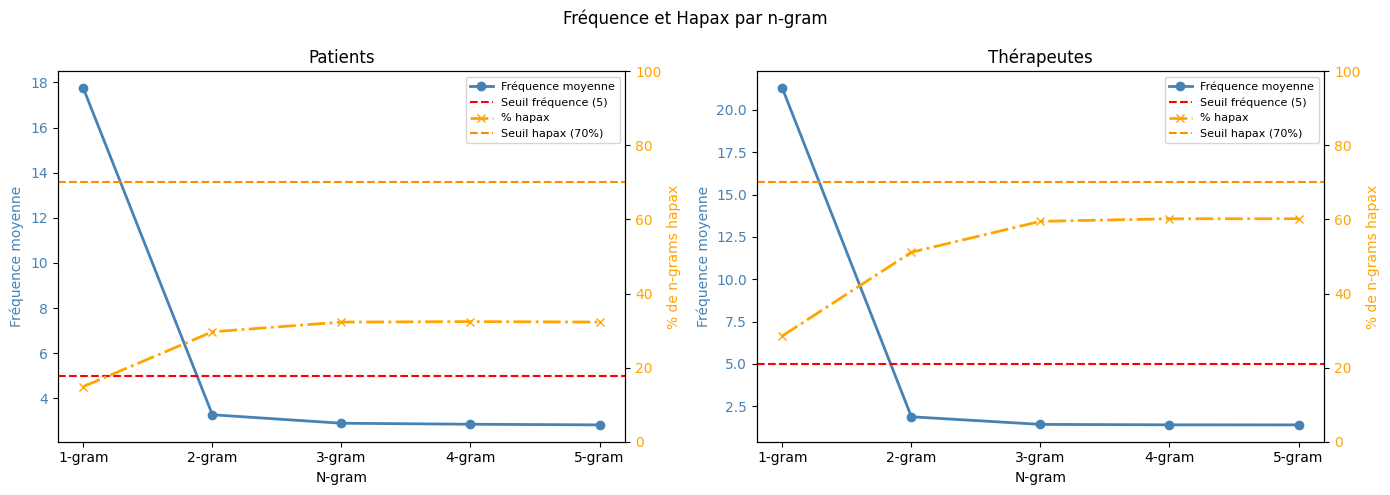
\includegraphics[width=1\textwidth]{graph_n_optimal.png}
\caption{Graphe de fréquence moyenne et pourcentage d'hapax en fonction de $n$}
\end{figure}

On remarque qu'à partir de $n = 1$, la fréquence diminue déjà fortement. Cependant,
les bigrams et trigrams restent exploitables car le seuil d'hapax n'est pas dépassé.

\pagebreak

\subsection{Résultats — Logan, Victor et Lucas}

Les bigrams et trigrams apportent un contexte nettement plus riche que les unigrams seuls.
Ils peuvent permettre par la suite d'identifier des patrons linguistiques et des thèmes récurrents
pour le topic modeling mais malheureusement leur fréquence est relativement faible,
ce qui rend leur exploitation plus délicate\dots


\vspace{10px}

\begin{table}[h]
\centering
\begin{tabularx}{0.65\textwidth}{lc||lc}
\toprule
\textbf{Unigram} & \textbf{fréquence} & \textbf{Unigram} & \textbf{fréquence}\\
\midrule
\textit{relationship} & 486 & \textit{help} & 2150\\
\textit{love} & 431 & \textit{relationship} & 1933\\
\textit{friend} & 369 & \textit{way} & 1668\\
\bottomrule
\end{tabularx}
\caption{Trois plus fréquent \textbf{unigram} pour les patients (gauche) et thérapeutes (droite)}
\end{table}

\vspace{10px}

\begin{table}[h]
\centering
\begin{tabularx}{0.65\textwidth}{lc||lc}
\toprule
\textbf{Bigram} & \textbf{fréquence} & \textbf{Bigram} & \textbf{fréquence}\\
\midrule
\textit{issue address} & 94 & \textit{therapist help} & 160\\
\textit{self esteem} & 65 & \textit{ask question} & 154\\
\textit{month ago} & 64 & \textit{mental health} & 153\\
\bottomrule
\end{tabularx}
\caption{Trois plus fréquent \textbf{bigram} pour les patients (gauche) et thérapeutes (droite)}
\end{table}

\vspace{10px}

\begin{table}[h]
\centering
\begin{tabularx}{0.9\textwidth}{lc||lc}
\toprule
\textbf{Trigram} & \textbf{fréquence} & \textbf{Trigram} & \textbf{fréquence}\\
\midrule
\textit{history sexual abuse} & 51 & \textit{hello thank question} & 68\\
\textit{low self esteem} & 50 & \textit{mental health professional} & 52\\
\textit{couple therapy session} & 48 & \textit{landwehr dbh lpc} & 51\\
\bottomrule
\end{tabularx}
\caption{Trois plus fréquent \textbf{trigram} pour les patients (gauche) et thérapeutes (droite)}
\end{table}

\bigskip

Maintenant que nous avons une idée des mots les plus fréquents, nous allons devoir identifier
les thématiques majeures abordées dans les conversations.
Pour cela, nous allons appliquer différentes méthodes de \textbf{topic modeling}, en comparant leurs avantages et limites respectifs.

\pagebreak

\chapter{Topic Modeling}

\section{Préambule}
Le \textbf{topic modeling} est une technique d'extraction de thèmes latents à partir d'un corpus de textes.
Il existe plusieurs méthodes pour réaliser cette tâche, chacune avec ses propres avantages et limites.
Dans cette section, nous allons présenter quatre approches différentes pour identifier les thématiques majeures dans les conversations de santé mentale, 
en commençant par une méthode manuelle basée sur un lexique personnalisé, puis en explorant des méthodes plus automatisées et robustes comme TF-IDF, Word2Vec et LDA.

\begin{note}[Remarque importante]
\textbf{Chaque membre de l'équipe a appliqué sa propre version de ces méthodes}, ce qui nous a permis d'avoir une diversité d'approches et de résultats à comparer.
Par question de clareté, nous allons présenter les résultats de chaque méthode de manière synthétique, en présentant les résultats les plus pertinents et en discutant de leurs avantages et limites respectifs.\\
(\textit{voir les notebooks\footnotemark{} individuels pour les détails de chaque implémentation}).
\end{note}
\footnotetext{\href{https://github.com/cypnet/Analyse-de-conversations-sur-la-sant-mentale/tree/main/notebooks}{Liens github des notebooks}}

\begin{table}[H]
\begin{center}
\begin{tabular}{@{}lL{6cm}@{}}
\toprule
\textbf{Méthode} & \textbf{Membres} \\
\midrule
Lexique personnalisé & Diogo, Trésor, Emin, Logan, Victor, Idir, Trésor, Yvan, Lucas \\
\midrule
TF-IDF + K-Means & Ulysse, Diogo, Trésor, Emin, Logan, Victor, Idir, Laure, Trésor, Yvan, Lucas\\
\midrule
Word2Vec + Clustering & Ulysse, Diogo, Trésor, Emin, Logan, Victor, Idir, Trésor, Yvan, Lucas \\
\midrule
LDA (Latent Dirichlet Allocation) & Ulysse, Diogo, Trésor, Emin, Logan, Victor, Idir, Trésor, Yvan, Lucas \\
\bottomrule
\end{tabular}
\caption{Répartition des méthodes de topic modeling entre les membres de l'équipe}
\end{center}
\end{table}

\pagebreak

\section{Méthode 1 : Lexique personnalisé}

\subsection{Principe}

Un dictionnaire thématique est construit \textbf{manuellement}, en associant chaque thème de santé mentale 
à une liste de mots-clés. Chaque question peut être assignée à plusieurs thèmes simultanément 
(classification multi-label).\\
Le but de cette première section était de nous introduire le principe de dictionnaire thématique,
ainsi que de nous familiariser avec les thématiques récurrentes dans les conversations de santé mentale.

\begin{note}[Remarque]
  Ce filtrage manuelle étant bien entendu subjectif, il ne sera pas appliqué dans les méthodes de topic modeling, qui sont plus robustes à ce type de bruit lexical.
\end{note}

Nous allons présenter deux exemples de lexiques, l'un minimaliste (Trésor) et l'autre plus étendu (Diogo). 
Bien entendu chaque membre de l'équipe a réalisé son propre lexique.

\subsection{Approche minimaliste (Trésor)}

\begin{lstlisting}
lexique = {
    'Anxiete':    ['anxious', 'anxiety', 'panic', 'fear'],
    'Depression': ['depress', 'depression', 'sad', 'suicide'],
    'Relation':   ['relationship', 'husband', 'wife', 'partner']
}
\end{lstlisting}

\subsection{Approche étendue (Diogo)}

\begin{lstlisting}
LEXICON = {
    'Anxiety':    ['anxiety', 'anxious', 'panic', 'worry', 'worried', 'nervous',
                   'fear', 'phobia', 'stress', 'stressed', 'overthink', 'dread'],
    # 11 autres thèmes contenant chacun 12 mots...
}
\end{lstlisting}

\pagebreak

\subsection{Résultats}

Les thèmes apparaissant de façon transversale :
\begin{itemize}
  \item \textbf{Anxiété} (\textit{anxiety}, \textit{panic}, \textit{stress})
  \item \textbf{Dépression} (\textit{depression}, \textit{sad}, \textit{hopeless})
  \item \textbf{Relations} (\textit{relationship}, \textit{love}, \textit{partner}) — thème le plus fréquent
\end{itemize}

\subsection{Évaluation critique}

\begin{center}
\begin{tabular}{@{}ll@{}}
\toprule
\textbf{Avantage} & \textbf{Limite} \\
\midrule
Très interprétable et explicable & Rigide : ne capte que les mots explicitement listés \\
Facile à adapter au domaine & Ne gère pas les synonymes non prévus \\
Résultats stables et reproductibles & Nécessite une expertise métier \\
Classification multi-label naturelle & Insensible au contexte d'usage d'un mot \\
\bottomrule
\end{tabular}
\end{center}

\bigskip

Toute l'équipe est en accord avec trois thématiques principales: anxiété, dépression et relations.
Or cela ne signifie pas que ses thématiques sont les plus fréquentes,
bien au contraire! D'autres thèmes bien plus spécifique auquels on ne pensserais pas peuvent faire leur apparition. 
D'où l'intérêt de méthodes plus robustes et moins sujetives que le lexique manuel. 

\pagebreak

\section{Méthode 2 : TF-IDF + K-Means}

\subsection{Principe de TF-IDF}

Le \textbf{TF-IDF} (\textit{Term Frequency — Inverse Document Frequency}) est une méthode
de pondération évaluant l'importance d'un mot au sein d'un document par rapport à l'ensemble
du corpus. Il combine deux composantes :

\begin{itemize}
  \item \textbf{Term Frequency (TF)} : fréquence d'un terme dans le document.
  $$tf_{i,j} = \frac{n_{i,j}}{\sum_k n_{k,j}}$$
  où $n_{i,j}$ est le nombre d'occurrences du terme $i$ dans le document $j$.

  \item \textbf{Inverse Document Frequency (IDF)} : pondération par la rareté du mot dans
  le corpus.
  $$idf(w) = \log\!\left(\frac{N}{df_t}\right)$$
  où $N$ est le nombre total de documents et $df_t$ le nombre de documents contenant le terme $t$.
\end{itemize}

Le score final est :
$$w_{i,j} = tf_{i,j} \times \log\!\left(\frac{N}{df_i}\right)$$

Les vecteurs sont ensuite normalisés par la norme L2 afin que la longueur des documents ne
biaise pas les comparaisons.

Grâce au pré-traitement déjà effectué (suppression des stopwords, lemmatisation), l'IDF
discrimine mieux les termes et les scores sont plus significatifs.

\subsubsection{Vectorisation TF-IDF}
On ne peut malheureusement pas utiliser TF-IDF directement sur les textes bruts, il faut d'abord les vectoriser.
Vectoriser un texte signifie le transformer en une représentation numérique, pour que par la suite les algorithme puisse les traiter.\\
Pour cela, nous allons utiliser la fonction \texttt{TfidfVectorizer} de la bibliothèque \textbf{scikit-learn}.
Cette fonction à de grand avantages, elle permet de:
\begin{itemize}
  \item lister tout les mots uniques
  \item définir le score TF
  \item définir le score IDF
  \item définir le score final et vecteur L2
\end{itemize}
\vspace{10px}

\begin{figure}[ht]
\centering
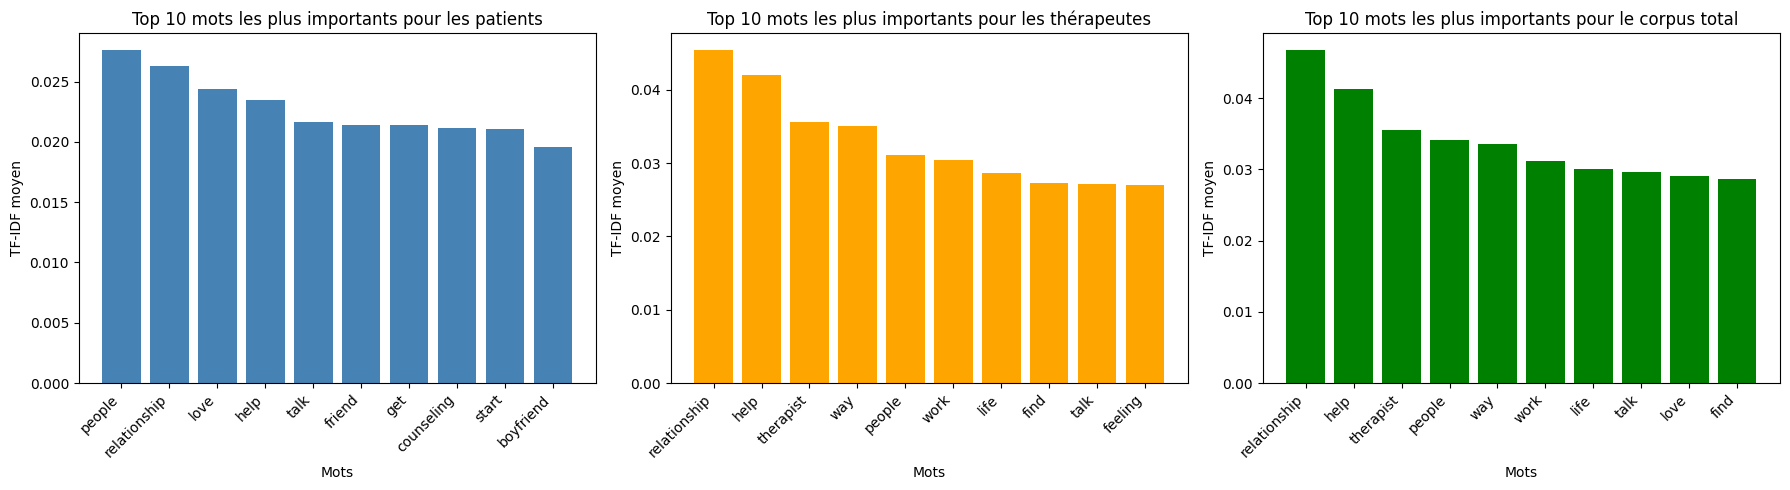
\includegraphics[width=\textwidth]{hist_tfidf_top_mot_important.png}
\caption{Exemple d'histogramme des 10 mots les plus importants selon le score TF-IDF (Logan)}
\end{figure}

\pagebreak

\subsubsection{Clustering K-Means}
Après avoir vectorisé les textes en utilisant TF-IDF, nous obtenons une matrice de taille $N \times M$ (où $N$ est le nombre de documents et $M$ le nombre de mots uniques).
Gràce à cette matrice, nous allons pouvoir maintenant regroupper les mots similaires en \textbf{clusters},
or nous devons dans un premier temps définir le nombre de clusters $K$ à utiliser.
Un des risques est de choisir un $K$ trop petit ou trop grand, 
ce qui peut conduire à des clusters peu significatifs ou à un sur-apprentissage.

\subsection{Sélection du nombre de clusters ($K$)}

Plusieurs stratégies explorées :
\begin{itemize}
  \item Définition manuelle
  \item Méthode du coude (\textit{elbow method})
  \item Équilibrage des tailles
\end{itemize}

\begin{note}[Remarque]
  Une méthode que nous aurions pu explorer mais que nous n'avons pas fait est la \textbf{silhouette score}, qui mesure la cohésion et la séparation des clusters pour différents $K$.
  Combiné avec la méthode du coude, cela aurait pu nous aider à trouver un compromis entre la qualité des clusters et leur interprétabilité.
\end{note}

\pagebreak

\subsection{Résultats selon $K$}

\subsubsection*{$K = 6$ — Clusters déséquilibrés — Logan}
La méthode du coude (\textit{elbow method}) a été utilisée pour déterminer le nombre optimal
de clusters $K$. L'inertie diminue fortement jusqu'à $K = 6$, puis la courbe se stabilise.

\begin{figure}[ht]
\centering
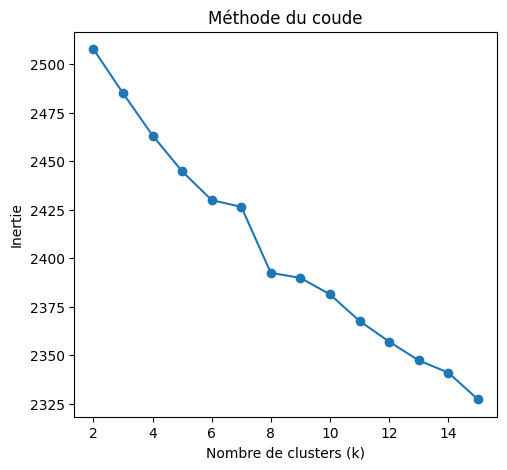
\includegraphics[width=0.45\textwidth]{graph_methode_coude.png}
\caption{Graphe de la méthode du coude pour déterminer le nombre optimal de clusters $K$}
\end{figure}

\textbf{K = 6 a donc été retenu.}
\begin{center}
\begin{tabular}{lr}
\toprule
\textbf{Thème identifié} & \textbf{Effectif} \\
\midrule
Dépression sévère — idées suicidaires & 457 \\
Mal-être général — perte de motivation & 112 \\
Dépression sévère — fatigue mentale & 46 \\
Thérapie de couple — anxiété & 223 \\
Traumatisme — abus — maladie grave & 1 718 \\
Problèmes familiaux — divorce — identité & 139 \\
\bottomrule
\end{tabular}
\end{center}

\begin{warn}[Résultat peu satisfaisant]
Fort déséquilibre de taille (46 vs 1 718), thèmes qui se recoupent.
Une des solutions aurait été d'agrandir la plage de $K$ testée, mais cela aurait conduit à des clusters encore plus petits et moins interprétables.
\end{warn}

\pagebreak

\subsubsection*{$K = 3$ — Meilleure configuration avec LSA — Diogo}

\textbf{Très petite explication du LSA}
% \begin{lstlisting}
% vec = TfidfVectorizer(
%     max_features=10000,
%     ngram_range=(1, 3),
%     min_df=3,
%     max_df=0.5,
%     sublinear_tf=True,
%     stop_words=list(STOPWORDS),
%     strip_accents="unicode",
%     token_pattern=r"(?u)\b[a-zA-Z]{2,}\b"
% )
% \end{lstlisting}

La \textbf{LSA} (\textit{Latent Semantic Analysis}) est une technique de réduction de
dimension appliquée à la matrice TF-IDF. Elle repose sur la \textbf{décomposition en
valeurs singulières} (SVD) :

$$M = U \cdot \Sigma \cdot V^\top$$

où $M \in \mathbb{R}^{d \times n}$ est la matrice terme-document ($d$ termes, $n$ documents),
$U$ les vecteurs de termes, $\Sigma$ la matrice diagonale des valeurs singulières, et $V^\top$
les vecteurs de documents dans l'espace latent.

En ne conservant que les $k$ premières composantes ($k \ll d$), on projette les documents
dans un espace sémantique réduit avec deux avantages principaux :

\begin{itemize}
  \item \textbf{Réduction du bruit lexical} : des termes synonymes (ex. \textit{sad} et
        \textit{depressed}) qui co-occurrent dans des contextes similaires se rapprochent
        dans l'espace réduit.
  \item \textbf{Amélioration du clustering} : K-Means est sensible à la \textit{malédiction
        de la dimensionnalité} ; réduire la dimension améliore la qualité des clusters.
\end{itemize}

Dans l'implémentation de Diogo, la LSA est appliquée via \texttt{TruncatedSVD} de
\texttt{scikit-learn} avec 50 composantes, après vectorisation TF-IDF :

\begin{lstlisting}
from sklearn.decomposition import TruncatedSVD
from sklearn.pipeline import make_pipeline
from sklearn.preprocessing import Normalizer

svd = TruncatedSVD(n_components=50, random_state=42)
X_lsa = make_pipeline(X)
X_norm = Normalizer().fit_transform(X_lsa) # Normalisation L2
\end{lstlisting}

La normalisation finale (norme L2) garantit que les distances cosinus restent interprétables
après la projection. Comme montré dans les résultats ($K = 3$), l'ajout de la LSA conduit à
des clusters plus équilibrés et thématiquement plus distincts par rapport au clustering TF-IDF seul.

Cela nous permet d'obtenir des clusters plus équilibrés et thématiquement plus distincts, couvrant 100\,\% du corpus.

\begin{center}
\begin{tabular}{@{}L{5cm}lrL{4cm}@{}}
\toprule
\textbf{Topic} & \textbf{Effectif} & \textbf{Part} & \textbf{Mots-clés principaux} \\
\midrule
Family and relational dynamics            & 309 & 38,8\,\% & friends, family, child, dad, mom, husband \\
Emotional distress and mental health      & 284 & 35,7\,\% & anxiety, depression, stop, start, school \\
Romantic relationships and intimacy       & 203 & 25,5\,\% & love, relationship, boyfriend, sex, girl \\
\bottomrule
\end{tabular}
\end{center}

Même si les résultats sont meilleurs, on observe que les thèmes restent assez larges et se recoupent partiellement (ex. \textit{family} peut apparaître dans les deux premiers clusters).

\subsection{Évaluation critique}

Bien que la méthode TF-IDF + K-Means soit rapide et facile à implémenter, elle présente plusieurs limites :

\begin{center}
\begin{tabular}{@{}L{7.5cm}L{7.5cm}@{}}
\toprule
\textbf{Avantage} & \textbf{Limite} \\
\midrule
Méthode rapide et scalable & Sensible au choix de $K$ \\
Bien documentée et reproductible & Ignore la sémantique contextuelle des mots \\
Compatible avec LSA pour de meilleurs résultats & Mots traités comme des entités indépendantes \\
\bottomrule
\end{tabular}
\end{center}

Ses limites peuvent être partiellement atténuées en combinant avec une réduction de dimension (LSA) ou en utilisant des représentations plus riches comme les word embeddings, \textbf{ce qui nous amène à la méthode suivante}.

\pagebreak

\section{Méthode 3 : Word Embeddings}

\subsection{Principe du Word Embedding}

Le \textbf{Word Embedding} (plongement lexical) est une représentation sémantique des mots
sous forme de vecteurs de nombres réels. Deux mots de sens proche ont des vecteurs proches
dans l'espace mathématique.

Contrairement à TF-IDF qui est une \textbf{représentation statistique} (fréquence d'apparition),
Word2Vec est une \textbf{représentation sémantique} : il apprend ce que le mot signifie en
observant les mots qui l'entourent dans le corpus. Ainsi, \textit{"sad"} et \textit{"depressed"}
se trouvent proches dans l'espace vectoriel parce qu'ils apparaissent dans des contextes
similaires.

\subsection{Skip-Gram vs CBOW}

Word2Vec propose deux architectures :
\begin{itemize}
  \item \textbf{CBOW} (\textit{Continuous Bag of Words}) : prédit le mot central à partir de
        son contexte. Très rapide sur les grands corpus, mais la moyenne du contexte
        \textit{lisse le bruit}, ce qui peut effacer des nuances importantes.
  \item \textbf{Skip-Gram} (\texttt{sg=1}) : prédit le contexte à partir du mot central.
        Plus adapté aux \textbf{corpus petits et spécialisés} car il génère plus d'exemples
        d'entraînement par mot, compensant le manque de données.
\end{itemize}

\begin{note}[Remarque]
  Étant donné que notre corpus est relativement \textbf{petit et spécialisé}, le mode \textbf{Skip-Gram est généralement recommandé}\footnote{Référence à cette décision: \href{https://www.geeksforgeeks.org/nlp/word-embeddings-in-nlp-comparison-between-cbow-and-skip-gram-models/}{geeksforgeeks.org}} 
  pour capturer des relations sémantiques plus fines.
\end{note}

\pagebreak

\subsection{Word2Vec (Skip-gram) — Logan}
La version de logan implémente Word2Vec en mode Skip-Gram, avec les hyperparamètres suivants:
\begin{itemize}
  \item \textbf{vector\_size=100} : chaque mot est représenté par un vecteur de 100 dimensions, ce qui permet de capturer une sémantique riche tout en restant gérable pour le clustering.
  \item \textbf{window=5} : le contexte de chaque mot est défini comme les 5 mots précédents et les 5 mots suivants, ce qui permet de capturer des relations à la fois locales et globales.
  \item \textbf{min\_count=3} : les mots apparaissant moins de 3 fois sont ignorés, ce qui réduit le bruit et améliore la qualité des embeddings.
  \item \textbf{epochs=10} : le modèle est entraîné pendant 10 itérations sur le corpus, ce qui permet d'obtenir des vecteurs stables sans sur-apprentissage.
  \item \textbf{seed=42} : pour assurer la reproductibilité des résultats.
  \item \textbf{sg=1} : pour activer le mode Skip-Gram, qui est plus adapté à notre corpus de taille modérée.
\end{itemize}

% \begin{lstlisting}
% model = Word2Vec(
%     sentences=all_sentences,
%     vector_size=100,
%     window=5,
%     min_count=3,
%     workers=4,
%     epochs=10,
%     seed=42,
%     sg=1               # Skip-gram
% )
% \end{lstlisting}

\subsubsection*{Résultats avec $K = 6$ (patients)}

\begin{center}
\begin{tabular}{llr}
\toprule
\textbf{Cluster} & \textbf{Thème} & \textbf{Effectif} \\
\midrule
0 & Dépression & 893 \\
1 & Problèmes sexuels — santé physique & 21 \\
2 & Thérapie de couple — anxiété & 414 \\
3 & Mal-être général & 1 084 \\
4 & Anxiété — trouble du sommeil & 195 \\
5 & Traumatisme & 88 \\
\bottomrule
\end{tabular}
\end{center}

Le problème que l'on pourrait avoir sur cette méthode est que les clusters sont très déséquilibrés, ce qui rend l'interprétation plus difficile.
La prochaine méthode que nous allons présenter, basée sur les \textbf{Sentence Transformers}, permet de mieux équilibrer les clusters et d'obtenir des thématiques plus distinctes.

\pagebreak

\subsection{Sentence Transformer (BERT / all-MiniLM-L6-v2) — Idir}

\subsubsection{Introduction rapide à BERT}
BERT (\textit{Bidirectional Encoder Representations from Transformers}) est un modèle de langage pré-entraîné développé par Google en 2018. 
Contrairement à Word2Vec, qui génère des embeddings statiques pour chaque mot, BERT produit des embeddings contextuels : le vecteur d'un mot dépend donc de la phrase dans laquelle il apparaît.

\begin{note}[Remarque]
Le modèle BERT, ayant sa partie dédié dans la troisièmre partie, sera expliqué bien plus en détails à ce moment là.
\end{note}

\subsubsection*{Résultats avec $K = 8$}

\begin{center}
\begin{tabular}{@{}cll@{}}
\toprule
\textbf{Effectif} & \textbf{Thème du cluster} & \textbf{Mots représentatifs} \\
\midrule
111 & Marriage and infidelity           & husband, married, relationship, love, wife \\
86  & Seeking therapy and abuse         & therapist, counseling, child, therapy, issues \\
121 & Romantic relationships and dating & love, relationship, boyfriend, guy, dating \\
101 & Family and parenting              & mom, dad, child, mother, family \\
95  & Anxiety and mental disorder       & anxiety, depression, attacks, sleep, panic \\
105 & Social anxiety and communication  & thoughts, friends, talking, upset, anger \\
75  & Sexuality and gender identity     & sex, girl, love, men, afraid, girls \\
102 & Depression and social life        & friends, school, sad, depressed, family \\
\bottomrule
\end{tabular}
\end{center}

\begin{note}[Remarque]
\textbf{Meilleur résultat} de la méthode 3 : clusters de taille homogène ($\approx$75--121), thèmes distincts et bien interprétables.
\end{note}

Les clusters obtenus avec les embeddings de BERT sont plus équilibrés et thématiquement plus distincts que ceux obtenus avec Word2Vec, 
ce qui confirme l'importance de la contextualisation dans la représentation des textes.
Une autre façon est d'obtenir des \textbf{embeddings de phrase} est d'utiliser les \textbf{embeddings moyennés de spaCy}, mais cela conduit à des résultats moins satisfaisants,
comme nous allons le voir dans la section suivante.

\pagebreak

\subsection{spaCy (embeddings moyennés) — Emin}

Dans cette approche, les embeddings de chaque mot sont extraits à l'aide de spaCy, puis moyennés pour obtenir une représentation vectorielle de chaque document.
Cependant, cette méthode présente plusieurs limites :
\begin{itemize}
  \item \textbf{Perte de contexte} : en moyennant les embeddings de tous les mots, on perd la structure syntaxique et les relations entre les mots, ce qui peut conduire à des représentations moins précises.
  \item \textbf{Mots peu informatifs} : les mots fréquents et peu discriminants (ex. \textit{know}, \textit{like}, \textit{feel}) peuvent dominer la représentation, masquant les thèmes plus spécifiques.
  \item \textbf{Résultats moins cohérents} : les clusters obtenus sont souvent moins thématiquement distincts et plus difficiles à interpréter que ceux obtenus avec des modèles plus avancés comme BERT.
\end{itemize}

\subsubsection*{Résultats avec $K = 5$}

\begin{center}
\begin{tabular}{ll}
\toprule
\textbf{Cluster} & \textbf{Mots principaux} \\
\midrule
0 & counseling, therapist, know, end, client, counselor \\
1 & dont, im, like, feel, know, want \\
2 & counseling, really, anything, help, people, something \\
3 & im, ive, like, feel, get, many \\
4 & feel, years, time, im, like, relationship \\
\bottomrule
\end{tabular}
\end{center}

\begin{warn}[Résultat insatisfaisant]
Clusters 0 et 2 très similaires, plusieurs clusters dominés par des mots peu informatifs.
\end{warn}

\subsection{Bilan comparatif — Méthode 3}

\begin{center}
\begin{tabular}{@{}llL{4cm}l@{}}
\toprule
\textbf{Modèle} & \textbf{Qualité} & \textbf{Points forts} & \textbf{Limites} \\
\midrule
Sentence Transformer & Très bonne & Contexte global, tailles homogènes & Modèle lourd \\
\midrule
Word2Vec (Skip-gram) & Bonne & Granularité thématique fine & Déséquilibre de taille \\
\midrule
spaCy & Passable & Rapide, simple & Perte de contexte \\
\bottomrule
\end{tabular}
\end{center}

L'équipe entière s'accorde pour dire que les embeddings de BERT (\textit{via Sentence Transformers}) offrent une meilleure qualité de clustering que les embeddings moyennés de spaCy ou les vecteurs Word2Vec,
grâce à leur capacité à capturer le contexte et les nuances sémantiques des textes.
Cependant, cette méthode est \textbf{plus lourde à entraîner et à utiliser}, ce qui peut être un frein pour des applications en temps réel ou sur des ressources limitées.
La dernière méthode que nous allons présenter, basée sur \textbf{LDA}, offre une approche différente en se concentrant sur la \textbf{modélisation thématique} plutôt que sur la représentation sémantique.

\pagebreak

\section{Méthode 4 : LDA (Latent Dirichlet Allocation)}

\subsection{Qu'est ce que le LDA ?}

Le \textbf{LDA} (\textit{Latent Dirichlet Allocation}) est un modèle génératif probabiliste
permettant de découvrir des sujets latents dans un corpus. C'est une approche bayésienne qui
suppose que chaque document est un \textbf{mélange de thèmes}, et que chaque thème est une
\textbf{distribution de mots}.

Contrairement à K-Means où chaque document appartient à un unique cluster, LDA assigne à
chaque conversation un mélange de thèmes avec des probabilités. Par exemple :

\begin{center}
\textit{"I feel sad and anxious"} $\longrightarrow$ 70\,\% dépression + 30\,\% anxiété
\end{center}

LDA produit deux sorties :
\begin{enumerate}
  \item \textbf{Thèmes $\to$ mots} : distribution des mots caractéristiques pour chaque thème.
  \item \textbf{Documents $\to$ thèmes} : proportion de chaque thème dans chaque conversation.
\end{enumerate}

\bigskip

Dans cette méthode, nous allons utiliser la bibliothèque \textbf{gensim} pour implémenter LDA, en utilisant les représentations de documents au format bag-of-words (corpus) et le dictionnaire de mots (id2word).
De plus, selon les membres, nous avons définit un nombre de thèmes $N\_TOPICS$ et un nombre de passes $PASSES$ pour l'entraînement du modèle.
\begin{figure}[ht]
  \begin{lstlisting}
    N_TOPICS = 6
    PASSES = 15
    
    model = LdaModel(
      corpus=corpus, 
      id2word=dictionary, 
      num_topics=n_topics, 
      random_state=42, 
      passes=passes
    )
  \end{lstlisting}
  \caption{Exemple d'implémentation de LDA avec la bibliothèque gensim — Logan}
\end{figure}

\pagebreak

\subsection{Résultats à 6 topics — Logan}

\begin{center}
\begin{tabular}{@{}ll@{}}
\toprule
\textbf{Thème} & \textbf{Mots représentatifs} \\
\midrule
Relations de couple et infidélité        & relationship, husband, child, listen, cheat, woman \\
Relations familiales et soutien social   & relationship, people, person, help, dad, family \\
Relations amoureuses et communication    & love, friend, talk, boyfriend, right, therapist \\
Anxiété et gestion émotionnelle          & anxiety, help, talk, friend, feeling, get, try \\
Détresse émotionnelle et conflits        & thought, boyfriend, girl, life, have, stop, cry \\
Thérapie et problématiques de couple     & normal, issue, wife, therapy, walk, couple, self \\
\bottomrule
\end{tabular}
\end{center}

\begin{note}[Interprétation]
Sur 6 topics, on retrouve des thèmes cohérents et distincts, couvrant les relations de couple, les relations familiales, l'anxiété, la détresse émotionnelle et la thérapie.
Cependant, certains thèmes se recoupent partiellement (ex. \textit{relationship} apparaît dans plusieurs topics), ce qui est une limite de l'approche.
\end{note}

\subsection{Résultats à 6 topics — Diogo}

\begin{center}
\begin{tabular}{@{}ll@{}}
\toprule
\textbf{Thème} & \textbf{Mots représentatifs} \\
\midrule
Romantic and sexual issues              & love, hes, sex, relationship, boyfriend \\
Mental health and disorders             & anxiety, depression, shes, boyfriend, mom \\
Therapy, communication and coping       & school, friends, right, high, live \\
Relationship trust and family           & girlfriend, thinking, hes, thoughts, stop \\
Intrusive thoughts and past             & mother, mom, dad, son, child \\
Family anger and conflict               & therapist, money, phone, relationship, friends \\
\bottomrule
\end{tabular}
\end{center}

\begin{note}[Interprétation]
Pour Diogo, les thèmes sont similaires à ceux de Logan, mais avec des nuances différentes. Par exemple, le thème "\textit{Therapy, communication and coping}" 
regroupe des mots liés à la vie quotidienne et à la gestion de l'anxiété, tandis que "\textit{Relationship trust and family}" met davantage l'accent sur les 
relations de confiance et les dynamiques familiales.
\end{note}

\pagebreak

\subsection{Résultats à 5 topics — Lucas}

\begin{center}
\begin{tabular}{@{}ll@{}}
\toprule
\textbf{Thème} & \textbf{Mots représentatifs} \\
\midrule
Santé mentale, sexualité et famille     & sexual, family, self, depression, married, anxiety \\
Relations amoureuses et questionnements & say, right, boyfriend, think, girlfriend, sex, love \\
Anxiété, vie quotidienne et thérapie    & think, boyfriend, couple, school, anxiety, therapy \\
Détresse émotionnelle et pensées nég.   & bad, think, sex, relationship, afraid, stop, love \\
Relations de couple et vie familiale    & boyfriend, make, counseling, child, life, talk \\
\bottomrule
\end{tabular}
\end{center}

\begin{note}[Interprétation]
Avec 5 topics, les thèmes sont plus larges et moins distincts que dans les configurations à 6 topics. Par exemple, le thème "\textit{Santé mentale, sexualité et famille}" 
regroupe des concepts très différents, ce qui rend l'interprétation plus difficile.
\end{note}

\subsection{Évaluation critique}
Lors de l'analyse des ses représentations thématiques, nous avons identifié plusieurs avantages et limites de la méthode LDA :

\begin{center}
\begin{tabular}{@{}ll@{}}
\toprule
\textbf{Avantage} & \textbf{Limite} \\
\midrule
Topics interprétables et cohérents       & Choix du nombre de topics difficile \\
Assignation douce = nuance inter-topics  & Sensible au prétraitement \\
Bien adapté aux textes courts            & Résultats variables selon hyperparamètres \\
Fondement probabiliste rigoureux         & Ne capture pas le contexte long \\
\bottomrule
\end{tabular}
\end{center}

\bigskip

Les résultats obtenues avec LDA sont généralement plus interprétables que ceux obtenus avec les méthodes basées sur les embeddings, car ils fournissent une distribution de mots pour chaque thème. 
Cependant, le choix du nombre de topics ($N\_TOPICS$) est crucial et peut grandement influencer la qualité des résultats. De plus, \textbf{LDA ne capture pas les relations à long terme entre les mots}, ce qui peut limiter sa capacité à identifier des thèmes plus complexes.

\smallskip
\textbf{Mais alors dans ce cas, quelle méthode est la meilleure?} Nous allons faire une conclusion comparée de toutes les méthodes présentées dans ce chapitre.

\section{Comparaison des méthodes}

\begin{center}
\renewcommand{\arraystretch}{1.3}
\begin{tabularx}{\textwidth}{@{}>{\raggedright\arraybackslash}p{2.6cm}>{\raggedright\arraybackslash}X>{\raggedright\arraybackslash}X>{\raggedright\arraybackslash}X@{}}
\toprule
\textbf{Méthode} & \textbf{Forces} & \textbf{Faiblesses} & \textbf{Usage recommandé} \\
\midrule
Lexique manuel
  & Interprétable, contrôlable
  & Rigide, non-généralisant
  & Catégorisation ciblée \\
\midrule
TF-IDF + K-Means
  & Rapide, scalable
  & Ignore le contexte
  & Exploration initiale \\
\midrule
Word2Vec
  & Similarités sémantiques
  & Déséquilibre possible
  & Représentation de mots \\
\midrule
Sentence Transformer
  & Contexte global, homogène
  & Lourd, moins interprétable
  & Meilleur clustering \\
\midrule
LDA
  & Assignation douce
  & Chevauchement de topics
  & Analyse thématique \\
\bottomrule
\end{tabularx}
\end{center}

\section*{Recommandation globale}

\begin{itemize}
  \item Pour \textbf{interpréter} les données : \textbf{LDA} est le plus lisible et le plus informativement riche.
  \item Pour \textbf{regrouper} les documents : \textbf{Sentence Transformer} (BERT) offre la meilleure qualité de clustering.
  \item Pour une \textbf{catégorisation stricte} : le \textbf{lexique manuel} reste le plus fiable si le domaine est bien défini.
\end{itemize}

\textbf{Que peut-on en conclure?} Il n'existe pas de méthode universelle pour l'analyse de texte, et \textbf{le choix dépend fortement des objectifs spécifiques, 
de la nature du corpus et des ressources disponibles}. Dans notre cas spécifique, la combinaison de plusieurs méthodes (ex. LDA pour l'analyse thématique + Sentence Transformer pour le clustering) 
pourrait offrir une approche plus complète et nuancée. 
Cepandant, cela nécessite une expertise plus approfondie et une validation rigoureuse pour éviter les biais et les interprétations erronées.

\chapter{Bilan de l'étape 1}

Cette première étape a permis de comprendre la structure du corpus et d'extraire les thèmes
principaux des conversations patient-thérapeute. Le pré-traitement rigoureux (filtrage des
langues, lemmatisation, stopwords) a été déterminant pour la qualité des résultats de topic
modeling.

Les différentes méthodes explorées (TF-IDF + K-Means, Word2Vec, Sentence Transformer, LDA) ont chacune leurs avantages et limites,
et ont permis d'obtenir des perspectives complémentaires sur les thèmes abordés dans les conversations.
Cependant, des problèmes techniques (hétérogénéité du nettoyage, gestion des doublons)
ainsi que des questions ouvertes (standardisation du nettoyage, identification des thérapeutes) 
restent à résoudre pour améliorer la qualité et la comparabilité des résultats.

Maintenant que nous avons une bonne compréhension des thèmes présents dans les conversations, 
nous allons pouvoir passer à l'étape suivante qui consiste à analyser les sentiments exprimés 
et à implémenter un système de question-réponse sur la santé mentale.

\chapter{Problèmes rencontrés et questions ouvertes}

\section{Problèmes techniques identifiés}

\begin{center}
\begin{tabularx}{\textwidth}{@{}>{\raggedright\arraybackslash}p{2.8cm}X X@{}}
\toprule
\textbf{Problème} & \textbf{Description} & \textbf{Impact} \\
\midrule
Hétérogénéité du nettoyage
  & Chaque membre a appliqué un pipeline différent
  & Résultats non directement comparables \\
Gestion des doublons
  & Nombre de patients variant de 796 à 995
  & Biais dans toutes les statistiques \\
Commentaires insuffisants
  & Manque de documentation dans les notebooks
  & Difficultés à comprendre le code des autres \\
Choix du nombre de clusters
  & Méthode du coude peu discriminante après $K = 6$
  & Difficulté à trouver un $K$ optimal \\
Normalisation des sorties
  & Formats de résultats différents entre membres
  & Comparaison manuelle laborieuse \\
\bottomrule
\end{tabularx}
\end{center}

\section{Questions ouvertes}

\begin{enumerate}
  \item \textbf{Standardisation du nettoyage} : nos moyennes de mots varient du simple au quadruple selon le niveau de filtrage. Faut-il fixer une règle commune ?
  \item \textbf{Gestion des doublons} : le nombre de patients varie de 796 à 995. Y a-t-il une consigne stricte sur la suppression des messages courts ou des doublons ?
  \item \textbf{Identification des thérapeutes} : existe-t-il une technique permettant de différencier les patients et thérapeutes entre eux sans identifiant ?
  \item \textbf{Mots semi-informatifs} : existe-t-il une méthode automatique pour traiter des mots moins significatifs que d'autres mais non considérés comme des stopwords standards ?
  \item \textbf{Sélection du nombre de clusters} : existe-t-il une méthode plus robuste que la méthode du coude pour déterminer automatiquement $k$ optimal ?
\end{enumerate}

% ══════════════════════════════════════════════════════════════════════════════
% PARTIE III : ÉTAPE 2
% ══════════════════════════════════════════════════════════════════════════════
\part{Étape 2 — Analyse et Accès aux conversations}

\chapter{Vue d'ensemble}

\section{Partie 1 : Analyse des sentiments des conversations}

\textit{Objectif : Implémenter un « catégoriseur » de sentiments des questions-réponses des thérapeutes selon une liste prédéfinie (Anxiété, Normal, Dépression, etc.).}

\textbf{Corpus d'entraînement} : \texttt{combined\_data.csv} (\textit{Sentiment Analysis for Mental Health}, Kaggle).

\textbf{Méthodologie} : Deux approches complémentaires :
\begin{itemize}
    \item \textbf{Méthode supervisée} (Naive Bayes, Régression Logistique, LinearSVC)
    \item \textbf{Méthode non supervisée} (K-Means)
\end{itemize}

\section{Partie 2 : Question-réponse sur la santé mentale}

\textit{Objectif : Implémenter un système de question-réponse simple sur le thème de la santé mentale.}

\textbf{Méthodologie} : Indexation du corpus de conversations, deux stratégies de recherche :
\begin{itemize}
    \item \textbf{Stratégie 1 — Similarité question-question}
    \item \textbf{Stratégie 2 — Similarité question-réponse}
\end{itemize}

\section{Répartition des tâches — Groupe 2 (Q/R)}

\begin{center}
\begin{tabular}{@{}lL{5.5cm}l@{}}
\toprule
\textbf{Sous-groupe} & \textbf{Méthode} & \textbf{Membres} \\
\midrule
Association mots-questions/réponses & Counter & Lucas \\
\midrule
Similarité question-question & Cosine similarity (TF-IDF+Word2Vec+BERT) & Yvan, Trésor \\
\midrule
Similarité question-réponse & Cosine similarity (TF-IDF+Word2Vec+BERT) & Idir, Laure \\
\bottomrule
\end{tabular}
\end{center}

\begin{figure}[H]
\begin{center}
\begin{tikzpicture}[
  scale=0.75,
  transform shape,
  node distance=8mm,
  >=Latex,
  box/.style={rounded corners, draw=blue!70!black, thick, fill=blue!5, align=center, text width=2.2cm, minimum height=0.9cm, inner sep=3pt, font=\small},
  method/.style={box, font=\footnotesize, text width=2cm, minimum height=0.8cm, node distance=4mm},
  group/.style={draw=red!75!black, rounded corners, dashed, inner sep=12pt, thick},
  subgroup/.style={group, draw=green!70!black, inner sep=8pt},
  arrow/.style={-Latex, thick, draw=blue!70!black},
  line/.style={thick, draw=blue!70!black}
]

  %=======================================

  % ETAPE 2 ==============================

  \node[box, text width=4cm] (step1) {Étape 1\\Exploration du jeu de données};
  \node[box, below=2cm of step1, text width=3cm] (conversations) {Analyse et accès\\aux conversations};
  \node[box, left=1cm of conversations, text width=3cm, yshift=-2cm] (conversationG1) {Analyse des sentiments\\des conversations};
  \node[box, right=1cm of conversations, text width=3cm, yshift=-2cm] (conversationG2) {Q/A sur la santé mentale};

  % Analyse des sentiments
  % Groupe 1
  \node[box, below=of conversationG1, xshift=-2.6cm](sentimentsG1) {Méthode supervisée};
  \node[method, below=of sentimentsG1, text width=3.5cm] (sg1m1) {Découpage\\train/validation/test};
  \node[method, below=of sg1m1, text width=3.5cm] (sg1m2) {Évaluation quantitative};
  \node[method, below=of sg1m2, text width=3.5cm] (sg1m3) {Prédiction sur dataset principal};
  % Groupe 2
  \node[box, below=of conversationG1, xshift=2cm, text width=2.6cm] (sentimentsG2) {Méthode\\non-supervisée};
  \node[method, below=of sentimentsG2, text width=3.5cm] (sg2m1) {Découpage\\train/validation/test};
  \node[method, below=of sg2m1, text width=3.5cm] (sg2m2) {Évaluation quantitative};
  \node[method, below=of sg2m2, text width=3.5cm] (sg2m3) {Prédiction sur dataset principal};
  % Annotation automatique
  \node[box, below=of sg2m3, xshift=-2.2cm, text width=3.6cm] (evalCateg){Évaluation catégoriseur};
  \node[box, below=of evalCateg, text width=3.5cm] (annotation) {Annotation automatique\\sur \textbf{train.csv}};
  % groupe Analyse des sentiments des conversations
  \node[group, fit=(conversationG1) (sentimentsG1) (sg1m1) (sg1m2) (sg1m3) (sentimentsG2) (sg2m1) (sg2m2) (sg2m3) (evalCateg) (annotation)] {};
  % sous-groupes Méthode supervisée et non-supervisée
  \node[subgroup, fit=(sentimentsG1) (sg1m1) (sg1m2) (sg1m3)] {};
  \node[subgroup, fit=(sentimentsG2) (sg2m1) (sg2m2) (sg2m3)] {};

  % Q&A
  \node[box, below=of conversationG2, xshift=1.5cm, text width=5cm](vectQA){Vectorisation (TF-IDF/Word2Vec/BERT)};
  % Groupe 1
  \node[box, below=of vectQA, text width=4cm] (qaG1) {Indexation du corpus\\(index inversé)};
  % Groupe 2
  \node[box, below=of qaG1, xshift=-2.2cm, text width=3.3cm] (qaG2) {Stratégie 1:\\Similarité Question-Question};
  \node[method, below=of qaG2](qaG2Test){Évaluation mini-test};
  % Groupe 3
  \node[box, below=of qaG1, xshift=2.2cm, text width=3.3cm] (qaG3) {Stratégie 2:\\Similarité Question-Réponse};
  \node[method, below=of qaG3](qaG3Test){Évaluation mini-test};

  \node[box, below=of qaG2Test, xshift=2.2cm, yshift=-3cm, text width=3.5cm] (filtrage) {Filtrage par sentiments};
  \node[box, below=of filtrage, text width=3.5cm] (resultats) {Réponses pertinentes};
  % groupe Q&A sur la santé mentale
  \node[group, fit=(conversationG2) (vectQA) (qaG1) (qaG2) (qaG2Test) (qaG3) (qaG3Test) (filtrage) (resultats)] {};
  % sous-groupes Indexation du corpus
  \node[subgroup, fit=(qaG2) (qaG2Test)] {};
  \node[subgroup, fit=(qaG3) (qaG3Test)] {};

  %LEGENDE
  % Group vide avec la signification à côté
  \node[group, below=2cm of annotation, minimum width=0.5cm, minimum height=0.5cm, xshift=-2.5cm] (g1) {};
  \node[right=0.5cm of g1, font=\footnotesize, color=blue!70!black] {Groupe de tâches};
  \node[subgroup, below=0.25cm of g1, minimum width=0.5cm, minimum height=0.5cm] (sg1) {};
  \node[right=0.5cm of sg1, font=\footnotesize, color=blue!70!black] {Sous-groupe de tâches};

  % Flèches du pipeline
  \draw[arrow] (step1) -- (conversations);
  % Groupe 1
  \draw[arrow] (conversations) -| (conversationG1);
  % Supervisée
  \draw[arrow] (conversationG1) -| (sentimentsG1);
  \draw[arrow] (sentimentsG1) -- (sg1m1);
  \draw[arrow] (sg1m1) -- (sg1m2);
  \draw[arrow] (sg1m2) -- (sg1m3);
  \draw[arrow] (sg1m3) |- (evalCateg);
  % Non-supervisée
  \draw[arrow] (conversationG1) -| (sentimentsG2);
  \draw[arrow] (sentimentsG2) -- (sg2m1);
  \draw[arrow] (sg2m1) -- (sg2m2);
  \draw[arrow] (sg2m2) -- (sg2m3);
  \draw[arrow] (sg2m3) |- (evalCateg);

  \draw[arrow] (evalCateg) -- (annotation);


  % Groupe 2
  \draw[arrow] (conversations) -| (conversationG2);
  \draw[arrow] (conversationG2.south) -| (vectQA);
  \draw[arrow] (vectQA) -- (qaG1);
  \draw[arrow] (qaG1) -| (qaG2);
  \draw[arrow] (qaG1) -| (qaG3);
  \draw[arrow] (qaG2) -- (qaG2Test);
  \draw[arrow] (qaG3) -- (qaG3Test);
  \draw[arrow] (filtrage) -- (resultats);

  % Flèche entre le groupe 1 et le groupe 2
  % Lier les flèches allant de annotation et qaG2Test/qaG3Test qui vont ensuite vers filtrage
  \draw[line] (annotation) -| (qaG2Test);
  \draw[line] (annotation) -| (qaG3Test);
  \draw[arrow] (annotation.east) -- ++(8.5,0) -| (filtrage.north);
  % Annotation sur la flèche
  \node[below=2pt of annotation.east, xshift=3.25cm, font=\footnotesize, color=blue!70!black] {fichier train.csv avec annotations};

  % flèche de sortie 
  \draw[arrow] (resultats) -- ++(0,-1.5) node[below, yshift=2pt, font=\footnotesize, color=blue!70!black] {résultats finaux};
  
  %=======================================

\end{tikzpicture}%
\label{fig:flowchart-etape2}
\caption{Pipeline détaillé de la seconde étape: Analyse et accès aux conversations}
\end{center}
\end{figure}

\chapter{Analyse des sentiments — Approches classiques}

\section{Méthodes supervisées}

Les modèles suivants ont été entraînés sur le corpus annoté :

\begin{center}
\begin{tabular}{lcc}
\toprule
\textbf{Modèle} & \textbf{Représentation} & \textbf{Accuracy test} \\
\midrule
Naive Bayes       & Bag-of-Words & 0,6666 \\
Naive Bayes       & TF-IDF       & 0,6927 \\
LinearSVC         & Bag-of-Words & 0,7309 \\
Logistic Regression & TF-IDF     & 0,7532 \\
LinearSVC         & TF-IDF       & 0,7586 \\
\bottomrule
\end{tabular}
\end{center}

\section{Méthode non supervisée (K-Means)}

\begin{center}
\begin{tabular}{lcc}
\toprule
\textbf{Modèle} & \textbf{Représentation} & \textbf{Accuracy test} \\
\midrule
K-Means & Word2Vec & 0,20 \\
K-Means & TF-IDF   & 0,4636 \\
\bottomrule
\end{tabular}
\end{center}

\chapter{Analyse des sentiments — Approches BERT}

\section{Qu'est-ce que BERT ?}

BERT (\textit{Bidirectional Encoder Representations from Transformers}) est un modèle de langage développé par Google en 2018. Il repose sur l'architecture Transformer et se caractérise par :
\begin{itemize}
    \item Sa \textbf{bidirectionnalité} : lecture du contexte dans les deux directions simultanément.
    \item Un \textbf{pré-entraînement} sur d'énormes corpus (Wikipedia, BooksCorpus) via deux tâches auto-supervisées : MLM (Masked Language Model) et NSP (Next Sentence Prediction).
    \item Un \textbf{fine-tuning} supervisé pour des tâches spécifiques.
\end{itemize}

\subsection{Tokenisation WordPiece}

\begin{lstlisting}[language={}]
"unhappiness"  ->  ["un", "##happi", "##ness"]
\end{lstlisting}

\subsection{Points forts}

\begin{itemize}
  \item Représentations contextuelles
  \item Transfert de connaissances efficace
  \item Écosystème riche (RoBERTa, DistilBERT, CamemBERT...)
\end{itemize}

\subsection{Limites}

\begin{itemize}
  \item Coût computationnel élevé (110M paramètres pour BERT-base)
  \item Limite de 512 tokens en entrée
  \item Complexité en $\mathcal{O}(n^2)$ par rapport à la longueur de la séquence
\end{itemize}

\section{Trois variantes BERT implémentées}

\begin{center}
\begin{tabular}{@{}llL{4cm}L{3cm}@{}}
  \toprule
  Modèle & Nom court & Description & Membres \\
  \midrule
  A & BERT sans fine-tuning & Extraction de features, poids gelés & Diogo \\
  B & BERT avec fine-tuning & Tous les poids mis à jour sur notre dataset & Diogo, Ulysse, Emin, Victor \\
  C & BERT spécialisé + fine-tuning & Modèle pré-entraîné sur des sentiments puis fine-tuné & Logan \\
  \bottomrule
\end{tabular}
\end{center}

\section{Modèle A — BERT sans fine-tuning}

\subsection{Principe}

Les poids de BERT sont gelés. BERT est utilisé comme extracteur de features, et une régression logistique apprend à partir des vecteurs \texttt{[CLS]} de 768 dimensions.

\subsection{Résultats — Diogo}

\begin{center}
\begin{tabular}{@{}lc@{}}
  \toprule
  \textbf{Modèle} & \textbf{Accuracy test}\\
  \midrule
  BERT sans fine-tuning & 0,7231 \\
  \bottomrule
\end{tabular}
\end{center}

\begin{center}
\begin{tabular}{@{}lccc@{}}
  \toprule
  Classe & Precision & Recall & F1-score \\
  \midrule
             Anxiety   &    0,73   &   0,67   &   0,70\\
             Bipolar   &    0,68   &   0,62   &   0,65\\
          Depression   &    0,64   &   0,70   &   0,67\\
              Normal   &    0,88   &   0,93   &   0,91\\
Personality disorder   &    0,56   &   0,38   &   0,45\\
              Stress   &    0,52   &   0,42   &   0,46\\
            Suicidal   &    0,65   &   0,59   &   0,62\\
  \bottomrule
\end{tabular}
\end{center}

\section{Modèle B — BERT avec fine-tuning}

\subsection{Principe}

Tous les poids de BERT sont mis à jour pendant l'entraînement. Une tête de classification (couche \texttt{Linear}) est ajoutée en sortie.

\textbf{Optimiseur} : AdamW avec learning rate de $2\times10^{-5}$.

\textbf{Scheduler} : \texttt{get\_linear\_schedule\_with\_warmup} pour décroître le learning rate linéairement.

\subsection{Résultats — Diogo, Ulysse, Victor, Emin}

\begin{center}
\begin{tabular}{@{}C{2cm}c@{}}
  \toprule
  \textbf{Epoch} & \textbf{Loss moyenne} \\
  \midrule
  1 & 0,6361 \\
  2 & 0,3871 \\
  3 & 0,2705 \\
  \bottomrule
\end{tabular}
\end{center}

\begin{center}
\begin{tabular}{@{}lc@{}}
  \toprule
  \textbf{Modèle} & \textbf{Accuracy test}\\
  \midrule
  BERT \textbf{avec fine-tuning} & \textbf{0,8302} \\
  \bottomrule
\end{tabular}
\end{center}

\begin{center}
\begin{tabular}{@{}lccc@{}}
  \toprule
  Classe & Precision & Recall & F1-score \\
  \midrule
             Anxiety   &    0,88   &   0,89   &   0,89\\
             Bipolar   &    0,86   &   0,85   &   0,86\\
          Depression   &    0,78   &   0,77   &   0,78\\
              Normal   &    0,95   &   0,95   &   0,95\\
Personality disorder   &    0,77   &   0,68   &   0,72\\
              Stress   &    0,73   &   0,76   &   0,74\\
            Suicidal   &    0,72   &   0,73   &   0,72\\
  \bottomrule
\end{tabular}
\end{center}

\section{Modèle C — BERT spécialisé + fine-tuning}

\subsection{Principe}

Utilisation d'un modèle déjà fine-tuné sur des tâches d'analyse de sentiments comme point de départ.

\subsection{Modèles disponibles sur Hugging Face}

\begin{center}
\begin{tabular}{@{}L{4.5cm}C{2cm}C{3.2cm}C{0.8cm}C{2cm}@{}}
  \toprule
  Identifiant HF & Base & Pré-entraîné sur\dots & Classes & Points forts \\
  \midrule
  \texttt{cardiffnlp/twitter-} \newline \texttt{roberta-base-sentiment} \newline \texttt{-latest} & RoBERTa & $\sim$124M tweets & 3 & Texte informel \\
  \texttt{nlptown/bert-base-} \newline \texttt{multilingual-uncased} \newline \texttt{-sentiment} & BERT multilingual & Avis produits & 5 & Multi-langue \\
  \texttt{siebert/sentiment-} \newline \texttt{roberta-large-english} & RoBERTa-large & 15 datasets & 2 & Généralisation \\
  \texttt{j-hartmann/emotion-} \newline \texttt{english-distilroberta} \newline \texttt{-base} & DistilRoBERTa & 6 datasets émotions & 7 & Émotions fines \\
  \bottomrule
\end{tabular}
\end{center}

\textbf{Modèle retenu} : \texttt{j-hartmann/emotion-english-distilroberta-base}, basé sur DistilRoBERTa et pré-entraîné sur 6 datasets d'émotions.

\subsection{Résultats — Logan}

\begin{center}
\begin{tabular}{@{}C{2cm}c@{}}
  \toprule
  \textbf{Epoch} & \textbf{Loss moyenne} \\
  \midrule
  1 & 0,6483 \\
  2 & 0,4305 \\
  3 & 0,3156 \\
  \bottomrule
\end{tabular}
\end{center}

\begin{center}
\begin{tabular}{@{}lc@{}}
  \toprule
  \textbf{Modèle} & \textbf{Accuracy test}\\
  \midrule
  BERT \textbf{spécialisé avec fine-tuning} & \textbf{0,8343} \\
  \bottomrule
\end{tabular}
\end{center}

\begin{center}
\begin{tabular}{@{}lccc@{}}
  \toprule
  Classe & Precision & Recall & F1-score \\
  \midrule
             Anxiety   &    0,87   &   0,90   &   0,88\\
             Bipolar   &    0,87   &   0,83   &   0,85\\
          Depression   &    0,80   &   0,76   &   0,78\\
              Normal   &    0,96   &   0,95   &   0,96\\
Personality disorder   &    0,69   &   0,73   &   0,71\\
              Stress   &    0,74   &   0,78   &   0,76\\
            Suicidal   &    0,71   &   0,76   &   0,73\\
  \bottomrule
\end{tabular}
\end{center}

\chapter{Comparaison globale — Analyse de sentiments}

\section{Tableau récapitulatif}

\begin{center}
\begin{tabular}{@{}L{4cm}C{2.5cm}C{3cm}L{3.5cm}@{}}
  \toprule
  Modèle & Accuracy test & Temps approx. & Remarque \\
  \midrule
  K-Means + W2V & 0,20 & Quelques minutes & Non supervisé \\
  K-Means + TF-IDF & 0,4636 & Quelques minutes & Non supervisé \\
  Naive Bayes + BoW & 0,6666 & Quelques secondes & Supervisé \\
  Naive Bayes + TF-IDF & 0,6927 & Quelques secondes & Supervisé \\
  LinearSVC + BoW & 0,7309 & Quelques minutes & Supervisé \\
  Logistic Regression + TF-IDF & 0,7532 & Quelques secondes & Supervisé \\
  LinearSVC + TF-IDF & 0,7586 & Quelques minutes & Supervisé \\
  \midrule
  BERT sans fine-tuning (A) & 0,7231 & Minutes (CPU) & Baseline BERT \\
  BERT avec fine-tuning (B) & 0,8302 & Heures (GPU) & Fine-tuning complet \\
  BERT spécialisé + FT (C) & 0,8343 & $\sim$30min (GPU) & Meilleur point de départ \\
  \bottomrule
\end{tabular}
\end{center}

\section{Conclusions}

\begin{enumerate}
  \item \textbf{Les modèles BERT surpassent largement les méthodes classiques} : gain d'environ 8 points de pourcentage.
  \item \textbf{L'apport du fine-tuning est significatif} : amélioration de plus de 10 points d'accuracy (Modèle A vs B).
  \item \textbf{Le gain du pré-entraînement spécialisé est marginal} : 0,8302 vs 0,8343, le fine-tuning sur notre dataset ayant déjà extrait des représentations efficaces.
  \item \textbf{Classes difficiles} : Depression et Suicidal restent souvent confondus, même par les modèles avancés. Personality disorder, Stress et Suicidal restent les classes les plus problématiques.
\end{enumerate}

\chapter{Système Question-Réponse}

\section{Indexation inversée}

L'indexation inversée associe chaque mot du corpus aux différentes questions et réponses dans lesquelles il apparaît.

\textbf{Formellement} : $\text{mot} \rightarrow \{(\text{question}, \text{réponse})\}$

Un compteur de type \texttt{Counter} est utilisé pour comptabiliser les occurrences des mots dans chaque discussion.

\section{Stratégie 1 : Similarité question-question}

Cette approche consiste à retrouver des réponses pertinentes à partir de la similarité entre la question de l'utilisateur et les questions présentes dans le corpus.

\textbf{Deux versions} :
\begin{itemize}
  \item \textbf{Version 1} : recherche sur l'ensemble du corpus
  \item \textbf{Version 2} : recherche limitée aux questions du même thème (filtrage par sentiment)
\end{itemize}

\textbf{Vectorisation} : TF-IDF, Word2Vec, BERT (all-MiniLM-L6-v2).

\textbf{Similarité} : cosinus, sélection des $k = 5$ questions les plus proches.

\section{Stratégie 2 : Similarité question-réponse}

Cette approche consiste à retrouver directement les réponses les plus pertinentes en se basant sur la similarité entre la question et l'ensemble des réponses du corpus.

\textbf{Deux versions} (avec et sans filtrage par thème).

\textbf{Mêmes méthodes de vectorisation et de calcul de similarité}.

\section{Évaluation des résultats}

Métrique : moyenne des inverses des scores de similarité cosinus sur 10 paires de test.

$$\text{Score} = \frac{1}{N} \sum_{i=1}^{N} \text{cosine\_similarity}(R_{\text{pred}, i}, R_{\text{true}, i})$$

\subsection{Version 1 — Sans filtrage par thème}

\begin{center}
\begin{tabular}{lccc}
\toprule
\textbf{Méthode} & \textbf{TF-IDF} & \textbf{Word2Vec} & \textbf{BERT} \\
\midrule
Similarité question-question & 0,3141 & 0,4242 & 0,4627 \\
Similarité question-réponse  & 0,32   & 0,53   & 0,5627 \\
\bottomrule
\end{tabular}
\end{center}

\subsection{Version 2 — Avec filtrage par thème (sentiment)}

\begin{center}
\begin{tabular}{lccc}
\toprule
\textbf{Méthode} & \textbf{TF-IDF} & \textbf{Word2Vec} & \textbf{BERT} \\
\midrule
Similarité question-question & 0,4101 & 0,622 & 0,67 \\
Similarité question-réponse  & 0,4101 & 0,664 & 0,702 \\
\bottomrule
\end{tabular}
\end{center}

\subsection{Analyse}

\begin{itemize}
  \item Les méthodes basées sur Word2Vec et BERT offrent de meilleures performances que TF-IDF.
  \item Le filtrage par thème améliore significativement les résultats (gain de 0,10 à 0,14).
  \item La stratégie question-réponse surpasse légèrement la stratégie question-question.
  \item BERT avec filtrage par thème obtient le meilleur score : 0,702.
\end{itemize}

% ══════════════════════════════════════════════════════════════════════════════
% PARTIE IV : CONCLUSION GÉNÉRALE
% ══════════════════════════════════════════════════════════════════════════════
\part{Conclusion générale}

\chapter{Synthèse des résultats}

\section{Étape 1 — Exploration du corpus}

L'exploration du corpus a révélé que :
\begin{itemize}
  \item Le corpus est centré sur les \textbf{relations interpersonnelles}, l'\textbf{anxiété} et la \textbf{dépression}.
  \item Les quatre méthodes de topic modeling sont complémentaires : LDA pour l'interprétation, Sentence Transformer pour le clustering, le lexique manuel pour la catégorisation stricte.
  \item Les divergences de prétraitement ont un impact significatif sur les résultats, soulignant la nécessité d'une standardisation.
\end{itemize}

\section{Étape 2 — Analyse de sentiments}

Les résultats montrent une progression claire :
\begin{itemize}
  \item Méthodes classiques : 66-76\% d'accuracy
  \item BERT sans fine-tuning : 72,31\%
  \item BERT avec fine-tuning : 83,02\%
  \item BERT spécialisé + fine-tuning : 83,43\%
\end{itemize}

Le gain apporté par BERT est considérable, mais les classes difficiles (Personality disorder, Stress, Suicidal) restent problématiques.

\section{Étape 2 — Système Question-Réponse}

Le système de question-réponse performe le mieux avec :
\begin{itemize}
  \item La stratégie \textbf{question-réponse} plutôt que question-question
  \item Les représentations \textbf{BERT} plutôt que TF-IDF ou Word2Vec
  \item Le \textbf{filtrage par sentiment} pour restreindre l'espace de recherche
\end{itemize}

Meilleur score obtenu : \textbf{0,702} (BERT, stratégie question-réponse, avec filtrage).

\chapter{Perspectives}

\begin{itemize}
  \item \textbf{Amélioration du prétraitement} : standardiser les pipelines de nettoyage pour garantir la comparabilité des résultats.
  \item \textbf{Augmentation des données} : explorer des techniques de data augmentation pour les classes sous-représentées (Personality disorder, Suicidal).
  \item \textbf{Modèles plus avancés} : tester des modèles plus récents comme RoBERTa-large, DeBERTa, ou des modèles génératifs.
  \item \textbf{Intégration complète} : fusionner le classificateur de sentiments et le système Q/R en un pipeline unifié.
  \item \textbf{Évaluation humaine} : compléter les métriques automatiques par une évaluation qualitative par des experts du domaine.
\end{itemize}

% ══════════════════════════════════════════════════════════════════════════════
% RÉFÉRENCES
% ══════════════════════════════════════════════════════════════════════════════
\chapter*{Références}
\addcontentsline{toc}{chapter}{Références}

\section*{Papiers de référence}

\begin{itemize}
  \item Thomas Hofmann (2013). \textit{Probabilistic Latent Semantic Analysis}. \\\url{https://arxiv.org/pdf/1301.6705}
  \item Devlin, J., Chang, M.-W., Lee, K., \& Toutanova, K. (2018). \textit{BERT: Pre-training of Deep Bidirectional Transformers for Language Understanding}. \\\url{https://arxiv.org/pdf/1810.04805}
  \item Wolf, T. et al. (2020). \textit{Transformers: State-of-the-Art Natural Language Processing}. \\\url{https://arxiv.org/pdf/1910.03771}
  \item Loshchilov \& Hutter (2019). \textit{Pre-Training and Fine-Tuning BERT for the IPU}. \\\url{https://docs.graphcore.ai/projects/bert-training/en/latest/bert.html}
\end{itemize}

\section*{Modèles Hugging Face}

\begin{itemize}
  \item \texttt{bert-base-uncased} \\\url{https://huggingface.co/google-bert/bert-base-uncased}
  \item \texttt{cardiffnlp/twitter-roberta-base-sentiment-latest} \\\url{https://huggingface.co/cardiffnlp/twitter-roberta-base-sentiment-latest}
  \item \texttt{j-hartmann/emotion-english-distilroberta-base} \\\url{https://huggingface.co/j-hartmann/emotion-english-distilroberta-base}
  \item \texttt{sentence-transformers/all-MiniLM-L6-v2} \\\url{https://huggingface.co/sentence-transformers/all-MiniLM-L6-v2}
\end{itemize}

\section*{Données}

\begin{itemize}
  \item Github — Page principal du projet \\\url{https://github.com/cypnet/Analyse-de-conversations-sur-la-sant-mentale}
  \item Github — Répertoire des notebooks \\\url{https://github.com/cypnet/Analyse-de-conversations-sur-la-sant-mentale/tree/main/notebooks}
  \item NLP Mental Health Conversations \\\url{https://www.kaggle.com/datasets/thedevastator/nlp-mental-health-conversations}
  \item Sentiment Analysis for Mental Health \\\url{https://www.kaggle.com/datasets/suchintikasarkar/sentiment-analysis-for-mental-health}
\end{itemize}

\section*{Outils}
\begin{itemize}
  \item Python 3.8+
  \item Bibliothèques : scikit-learn, transformers, sentence-transformers, pandas, numpy, matplotlib, seaborn
  \item Environnement : Jupyter Notebook, Google Colab
\end{itemize}

\end{document}